\section{Theoretical foundations}
The following sections are excerpts from papers (1)-(4), and not necessarily coherent.

\subsection{Elastodynamic equations of motion: weak form}
For the remainder of this paper, we will treat a non-rotating,
non-gravitating, isotropic (Lam\'{e} parameters $\lambda$, $\mu$)
earth model. The 3-D elastodynamic weak form comprises the following
three integral equalities for the displacement-potential vector
$(\bu,\chi)$ in an appropriate space with square-integrable derivatives
for all admissible test or trial functions $(\bw,w)$ \citep{nissen+:07a}:
%
\eqa \label{eq:weak1}
\lefteqn{0=\int_{\rm SIC}\rho\hspace{0.1em}\bw\cdot\ddot{\bu}\,d^3\bx
-\int_{\rm ICB}(\brh\cdot\bw) \ddot{\chi}\,d^2\bx +
}
\nonumber\\
\lefteqn{\hspace{1.5em}
\int_{\rm SIC}\left\{\lambda(\bdel\cdot\bw)
(\bdel\cdot\bu)
+\mu\bdel\bw\!:\!\left[\bdel\bu+\left(\bdel\bu\right)^T\right]\right\}
\,d^3\bx,
}
\ena
%
\eqa \label{eq:weak2}
\lefteqn{0=\int_{\rm FOC}\kappa^{-1}w\hspace{0.1em} \ddot{\chi}\,d^3\bx
+\int_{\rm ICB}w(\brh\cdot\bu)\,d^2\bx -
%}\nonumber\\
%\lefteqn{\hspace{0.5em}
\int_{\rm CMB}w(\brh\cdot\bu)\,d^2\bx
+\int_{\rm FOC}\rho^{-1}\bdel w\cdot\bdel\chi\,d^3\bx,}
\ena
%
\eqa \label{eq:weak3}
\lefteqn{\left\{
\begin{array}{c}
\bph\cdot\bw(r_{\rm r}\hspace{0.1em}\bzh)\delta(t)
\\ \bM:\bdel\bw(r_{\rm s}\hspace{0.1em}\bzh)H(t)
\end{array}\right\}=
%}\nonumber\\ \lefteqn{\hspace{0.5em}
\int_{\rm SMC}\rho\hspace{0.1em}\bw\cdot
\ddot{\bu}\,d^3\bx+\int_{\rm CMB}(\brh\cdot\bw)
\ddot{\chi}\, d^2\bx +}\nonumber\\
\lefteqn{\hspace{11.5em}\int_{\rm SMC}
\left\{\lambda(\bdel\cdot\bw)(\bdel\cdot\bu)
+\mu\bdel\bw\!:\!\left[\bdel\bu+\left(\bdel\bu\right)^T\right]\right\}d^3\bx}
\ena
%
where $\rho$ is the mass density, $\kappa$ the incompressibility,
$\bph\delta(t)$ the impulsive unity single-force vector acting at the
receiver at axial radius $r_{\rm r}$ and
$\bM H(t)$ the moment tensor at the source at axial radius $r_{\rm s}$ as a
step function in time, and second time derivatives are abbreviated as
$\ddot{\chi}=\partial^2_t{\chi}$.
The regions solid inner core SIC, fluid outer core FOC, and solid mantle and
crust SMC in eqs~(\ref{eq:weak1})--(\ref{eq:weak3}) are coupled by virtue of
the boundary surface integrals over the inner-core (ICB) and core-mantle
boundary (CMB). The fluid region eq.~(\ref{eq:weak2}) is treated via a
displacement potential formulation \citep{nissen+:07a}
%
\eq\label{eq:potential}
\bu=\rho^{-1}\bdel\chi,
\en
%
such that the fluid-domain wave equation becomes
\eq\label{eq:fluid_waveequation}
\kappa^{-1}\ddot{\chi}=\bdel\cdot(\rho^{-1}\bdel\chi).
\en
%
Note that the inclusion
of the inverse density in this definition of the potential $\chi$ results in
boundary integrals in eqs~(\ref{eq:weak1})--(\ref{eq:weak3}) that are
independent of any intrinsic material properties.
This is slightly different from other spectral-element methods
\citep{KoTr02a,manu04} in which the density-free potential leads
to solid-fluid boundary terms that depend on the discontinuity jumps.
This is necessitated by their inclusion of gravitation, but in our
non-gravitating case it is indeed feasible to pursue this convenient definition
in eq.~(\ref{eq:potential}).
For spherically symmetric background models, the 3-D weak system
eqs~(\ref{eq:weak1})--(\ref{eq:weak3}) may be reduced to its 2-D equivalent
by factorizing $(\bu,\chi)$ and $(\bw,w)$ into their $(s,z)$ and $\phi$
dependencies and analytically evaluating the longitudinal integrals
such as $\int_0^{2\pi}\sin^2{\phi}\,d\phi=\pi$ as shown by
\citet[][Section~4.4]{nissen+:07a}.
%
While retaining the $(s,\phi,z)$ cylindrical coordinate
system for the monopole and quadrupole cases, we develop the dipole system
in the $(+,-,z)$ system, such that
%
\eqa
\lefteqn{u_{\pm}(s,z)=\textstyle{\frac{1}{2}}[u_s(s,z)\pm u_{\phi}(s,z)],}\\
\lefteqn{w_{\pm}(s,z)=\textstyle{\frac{1}{2}}[w_s(s,z)\pm w_{\phi}(s,z)], }
\ena
%
inasmuch as this enables easier implementation of
the axial boundary conditions given by
\eqa
\lefteqn{\begin{array}{ll}
\textrm{Monopole:} &
\left(u_s=w_s\right)_{s=0}=0, \label{eq:ax_bc_mo}\\
\textrm{Dipole:}&
\left(u_-=w_-=u_z=w_z\right)_{s=0}=0, \label{eq:ax_bc_di}\\
\textrm{Quadrupole:}&
\left(u_s=w_s=u_\phi=w_\phi=u_z=w_z\right)_{s=0}=0
\label{eq:ax_bc_qu}.
\end{array}}
\ena
%

\subsection{Meshing}
\begin{figure*}[htb!]
\begin{center}
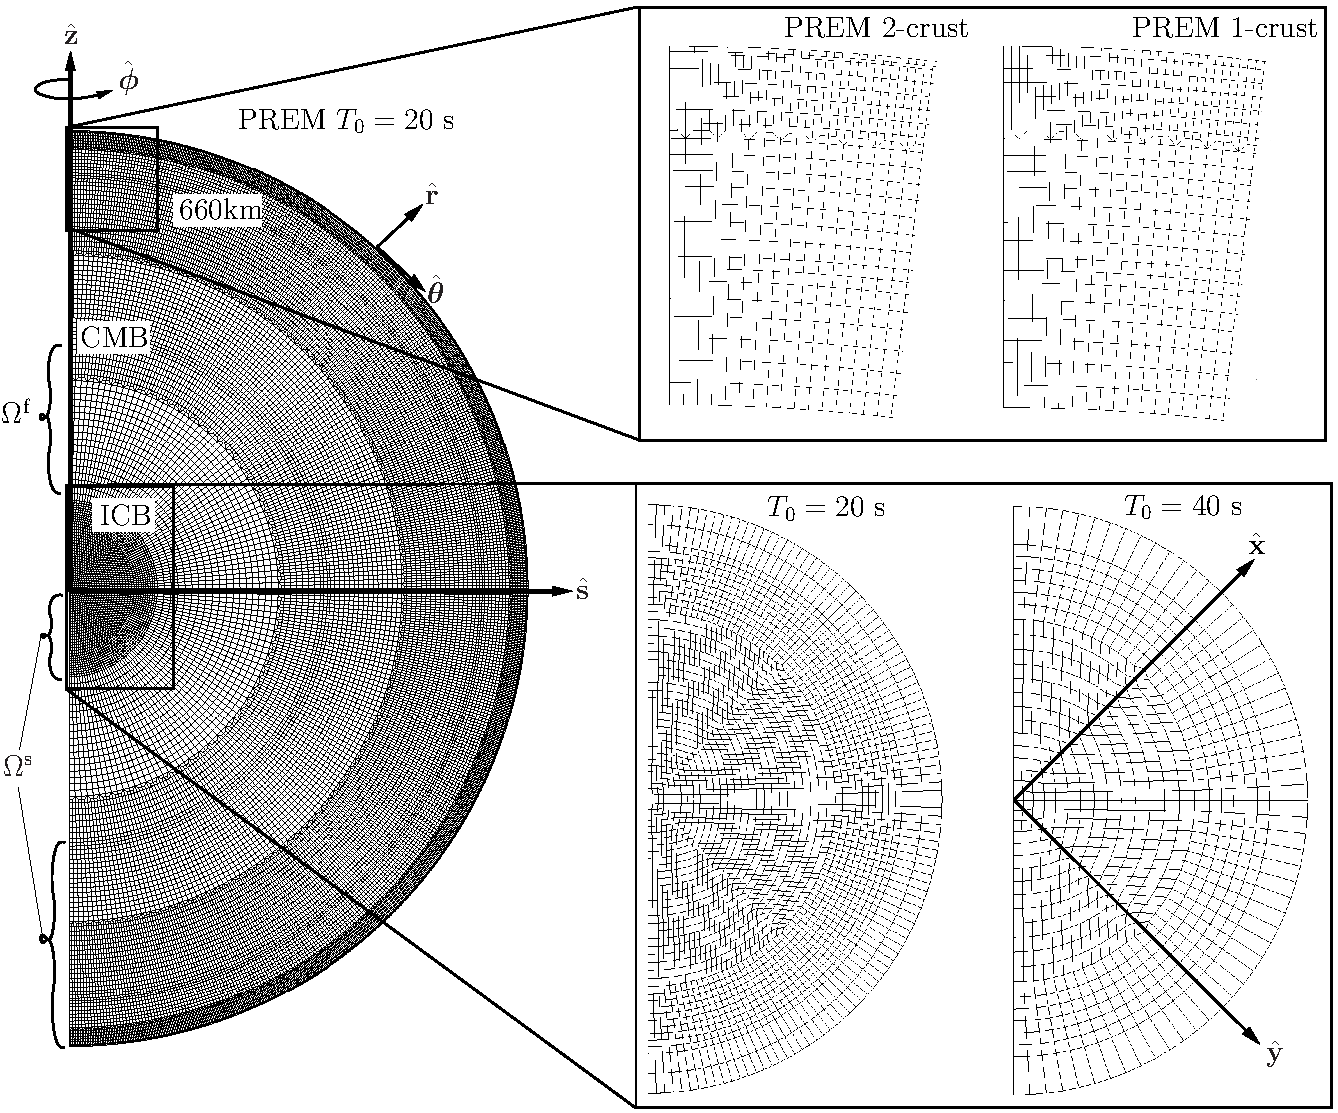
\includegraphics[scale=0.68]{prem_mesh.eps}
\caption{\textbf{Left:} The semicircular, solid-fluid
domain $\Omega=\Omega^{\rm s} + \Omega^{\rm f}$
discretized for the PREM background model using
quadrilateral elements $\Omega_e$ for dominant source period $T_0=20\, \textrm{s}$.
Note that all discontinuities are honored and several
conforming coarsening levels are included to maintain a relatively
constant resolution throughout the domain.
\textbf{Top right:} Enlargement of the crust for one (right) and two (left) crustal
layers, and the upper mantle, including one mesh coarsening region.
Note the variable vertical spacing due to discontinuities.
\textbf{Bottom right:} The central region for two resolutions.
To circumvent the singularity at the center,
we apply the following analytical expressions to reshape rectangular elements:
$\left|{x}\right|^p+\left|{y}\right|^p=\left|{r}\right|^p$,
$x=s+z,\,y=s-z,\,1\le p \le 2$.
This guarantees an easy handle on grid spacing which varies maximally
at the outermost, deformed elements of this central region and hence
controls stability and resolution.}
\label{img:prem_mesh}
\end{center}
\end{figure*}

Let us first define some geometric notation. As shown in
Fig.~\ref{img:prem_mesh} on the left, we work in a semi- disk
$\Omega=\Omega^{\rm s} + \Omega^{\rm f}$ of outer
radius $r_0$ spanned by $\bxh^{\rm 2D}=\bsh + \bzh=\brh+\bthetah$,
where $s\in [0,r_0]$, $z\in [-r_0,r_0]$ refer to cylindrical coordinates, and
radius $r\in [0,r_0]$ and colatitude $\theta\in [0,\pi]$ denote the spherical system.
The longitude $\phi\in [0,2\pi[$ is identical for both coordinate systems,
$\bxh^{\rm 3D}=\bxh^{\rm 2D}+\bphih$.  Material properties are invariant in
$\phi$, and the seismic wavefields either invariant (monopole sources) or analytically
continued from the $(s,z)$ plane \citep{nissen+:07a}; as a result we do not need
to discretize this third dimension. The grid structure represents the tiling into
non-overlapping solid ($\Omega_e^{\rm s}$) and fluid ($\Omega_e^{\rm f}$)
elements within which functions are analytically mapped to a reference square
$[-1,+1]^2$ to be expanded upon a polynomial basis
(see Section~\ref{section:spatial_discretization}).
Fig.~\ref{img:prem_mesh} also depicts magnified regions, showing
the crust and upper mantle (top right panel) for a two-layered PREM \citep{prem}
crust (left) and a one-layered ``crust'' (right). Note the variable vertical spacing due to the
discretization of adjacent discontinuities such as $600\,\textrm{km}$ and
$660\, \textrm{km}$.

The generation of a tangible mesh is no trivial matter.
In global seismology, we face the additional complication that the seismic
velocity $v_{\rm p,s}(r)$ generally increases, while horizontal grid spacing
(for spheroidal topologies) decreases with depth which works
as a doubly detrimental effect for meshing purposes.
Thus, we need to employ mesh coarsening to remediate these issues.
Additionally, a spheroidal grid cannot account for the
center of the sphere such that one needs to introduce a different (e. g. linear) topology.
The following factors also need to be considered as specific constraints
\citep[see also][Sections~3.1 and 4.1]{nissen+:07b}:
%
\begin{enumerate}
\item Quadrilateral element shapes,
\item Non-overlapping element boundaries,
\item Discontinuities to coincide with element boundaries.
\end{enumerate}
%
Point (i) is a minor issue inasmuch as the nature of
sharp global boundaries is spherical, i.e. mildly deformed and we do not
need to accommodate sharp wedges such as in regional velocity models which may
considerably influence the spacing variability and accuracy. Unless the
expensive mortar element method \citep{manu03}
or a discontinuous Galerkin approach based on numerical fluxes
\citep{KaeserDumbser:05} are used,
constraint (ii) only permits conforming coarsening architectures
\citep{KoTr02a}, which is what we chose \citep{nissen+:07b}.
Due to the last point (iii), however, we are faced with problems
such as discretizing the thin crustal layers even for long periods, thus
introducing local oversampling, or the existence of the fluid outer core, and
drastic velocity changes across the inner-core boundary
(see Section~\ref{section:central_region}).
For elastic wave phenomena, one seeks a discretization in which the local
$P$- or $S$-velocity-dependent wavelength $\Lambda(v_{\rm p,s}(r))$ is
sampled by a minimal variation in the number of grid points per wavelength $n_\Lambda$
anywhere in the spatial domain, and, simultaneously, minimal variation
in the number of time samples $T_0/\Delta{t}$ for the source-induced,
constant dominant (i.e., peak spectrum) period $T_0=\Lambda(v(r))/v(r)$.
The limiting values for the number of grid points per
wavelength, $n_\Lambda^0=\min{\left[n_\Lambda (r,\theta)\right]}$, controlling the
resolution, and the Courant number,
${\mathcal C}^0=\max{\left[{\mathcal C}(r,\theta))\right]}$, controlling the stability,
are inherent properties of the numerical scheme.
They are related to $T_0$ and $\Delta t$ via the
characteristic lead time $\tau_{\rm p,s}(r,\theta)=\Delta x(r,\theta)/v_{\rm p,s}(r)$
\footnote{Subscripts p,s are mnemonic indicators for adhering to the respectively
largest and smallest velocities for a given location; $\tau_{\rm s}$ in the fluid for example
is obviously defined by the overarching $P$-wave velocity, and near the surface by surface
wave velocities.}:
%
\eqa
\lefteqn{T_0 =n_\Lambda^0 \max{\left[\tau_{\rm s}(r,\theta)\right]},} \label{eq:period}\\
\lefteqn{\Delta{t}= {\mathcal C}^0 \min{\left[\tau_{\rm p}(r,\theta)\right]},}\label{eq:timestep}
\ena
%
where for each element, grid spacing $\Delta x(r,\theta)$ also depends on $\theta$ due to the
irregular Gauss-Lobatto-Legendre point distribution across elements \citep{nissen+:07b},
the occurrence of coarsening levels and the linear discretization of the central region.
Meshing in light of these constraints and ideas
principally aims at simultaneously
accommodating two factors:
(i) obtaining a smallest possible total number of elements, i.e. minimizing
the run-time memory cost with
(ii) the least variation in $\tau_{\rm p,s}(r,\theta)$.
This non-unique meshing procedure can be addressed from many angles.
%
\subsubsection{The background-model based spherical mesh}
%
Given the above constraints and the two-dimensional geometry,
we chose a straightforward approach to define our mesh:
Given an anticipated dominant period $T_0$
to be resolved, the minimal number of grid points per wavelength $n^0_\Lambda$,
and the location and velocity jump across discontinuities,
we calculate the maximally allowed, smallest global grid spacing
$\Delta x(\bx_{\rm minx})=T_0/n^0_\Lambda v_{\rm s}(r_{\rm minx})$  for that location
$\bx_{\rm minx}$ (typically just below the inner-core boundary, or at the surface).
We determine the exact lowermost radius $r_{\rm sl}$ of the spheroidal domain
(which characterizes the transition to rectangular element shapes)
by assuming that velocities within the inner core vary very little, starting with
the grid-spacing constraint $r_{\rm sl}\le r_{\rm minx}$ and moving to
the next possible lower radius
$r_{\rm sl}=\min\left[r_{\rm icb},{\rm int}\left(r_{\rm minx}/\Delta x(\bx_{\rm minx})\right)\right]$.
Additionally given the number of coarsening levels based
on the overall change in velocity, and the number of processors $N_{\rm proc}$
(see Section~\ref{section:parallel}), we obtain a permissible number of lateral
elements at the surface with grid spacing $\Delta x_{\rm lat}(r_0)$
upon adjusting $\Delta x(\bx_{\rm minx})$ such that
$\pi r_0$ is an even multiple of $N_{\rm proc} \Delta x_{\rm lat}(r_0)$.
Progressively moving downwards from the surface while honoring all
discontinuities and keeping vertical spacing between them similar to
the ideal value $T_0/n^0_\Lambda \min[v_{\rm s}(r)]$, a coarsening depth
$\textstyle{r_{\rm c}^i}$ is
found once $\textstyle{2\tau_{\rm s}(r_{\rm c}^i,\theta)\le T_0/n^0_\Lambda}$,
i.e. the spacing-velocity combination small enough to double and still resolve $T_0$.
Once this process is completed, the global time step is found given the limiting
Courant number ${\mathcal C}^0$ and $\min[\tau_{\rm p}]$ from the newly
created mesh.
For the SEM, the minimal possible number of points per wavelength is
$n_\Lambda^0\approx4$ \citep[e.g.][]{Ampuero+:07}, whereas ${\mathcal C}^0$ is
usually determined empirically and depends on the type and
order of the time extrapolation scheme (see Section~\ref{section:time_scheme})
and model-space dimension.
We obtain stable, accurate simulations up to ${\mathcal C}^0=0.6$, but one should
treat this choice carefully for each different mesh and time scheme
(see Section~\ref{section:time_scheme}).
Clearly, for any mesh containing model property or grid spacing variations,
these values for $\Delta{t}$ and $T_0$ are the global worst-case combinations,
and the actual, local Courant number and number of grid points per wavelength are
variable across the mesh. It is therefore our maxime to construct $\Delta x(r,\theta)$
in a way to minimize such variations. All applications in this paper are undertaken
with a polynomial order $N_{\rm pol}=4$, i.e. having $5$ grid points within an element
along a given dimension (including its edges); for a more thorough quantification of
meshing one may however also vary the polynomial order. Note that small polynomial
orders ease the meshing process in two ways: the smallest grid spacing within elements
upon a Gauss-Lobatto-Legendre basis varies as $N^{-2}_{\rm pol}$, and, secondly,
smaller element sizes allow for easier adaptation to material interfaces, especially
regarding closely spaced discontinuities like in the crust.
Fig.~\ref{img:prem_mesh} shows an example of a PREM model discretization using
this method for $T_0=20 \, \textrm{s}$ (left), and two magnified regions of interest, i.e.
the crust and upper mantle (top right) and the central region
(bottom right, see next section). Clearly, lower resolutions (being confronted with
the same background model as higher resolution realizations), are
less effective and expose larger spacing variations, as seen in the crust.
It is noteworthy to highlight that meshing is done only upon the lowest velocities
(surface waves near the surface, $S$ waves in deeper solid, $P$ waves in fluid), but one
subsequently determines the time step (i.e. the other component of the cost of the
scheme besides the number of elements ) based on largest ($P$ wave) velocities.

\begin{figure*}[t!]
\begin{center}
\includegraphics[scale=0.7]
{char_times_fig.eps}
\caption{Elementally minimal and maximal characteristic lead times scaled by
the time step and Courant number,
$\tau_{\rm p,s} {\mathcal C}^0/\Delta{t}$ in the spherical part of the model space as
a function of radius.
We depict PREM meshes for source periods $T_0=10\,\textrm{s}$ (left) and
$T_0=20\, \textrm{s}$ (right). The vertical line to the left
denotes unity, i.e. minimal possible $\min[\tau_{\rm p}]$ due to the definition of $\Delta{t}$ in
eq.~(\ref{eq:timestep}), and the vertical line to the right the corresponding maximal
value given by the relationship for the source period, eq.~(\ref{eq:period}), i.e.
$T_0 {\mathcal C}^0/(n^0_{\Lambda}\Delta{t})$.}
\label{img:char_time}
\end{center}
\end{figure*}
%
It is thus desirable to at least assess this entirely non-unique, potentially iterative process
a posteriori in terms of efficiency and overall cost.
In the interest of generality, we present examples of different mesh
realizations in terms of non-dimensionalized parameters, namely the
characteristic lead time
%
\eq
\frac{\tau_{\rm p,s}}{\min[\tau_{\rm p}]}=\tau_{\rm p,s}\frac{{\mathcal C^0}}{\Delta{t}},
\en
%
and the local oversampling ratio
%
\eq
\frac{T_0}{\Delta{t}^{\rm eff}(\bx)}=\frac{T_0}{n_\Lambda^0\tau_{\rm p}(\bx)}.
\en
%
\begin{table*}[htb!]
\begin{center}
\caption{Characteristic lead times and time steps for various mesh resolutions and Courant
number ${\mathcal C}^0=0.6$ and $n_\Lambda^0=6$.}
\label{table:char_time}
\begin{tabular}{@{}cccccccc}
\hline\hline
$T_0\, [s]$ & $\min{\left(\tau_{\rm p}^{\rm lat} \right)}\,[{\rm s}]$ &
$\min{\left(\tau_{\rm p}^{\rm rad} \right)}\,[{\rm s}]$ &
$\max{\left(\tau_{\rm s}^{\rm lat} \right)}\,[{\rm s}]$ &
%$\max{\left(\tau_{\rm s}^{\rm rad} \right)}\,[{\rm s}]$ &
$\Delta t\,[{\rm s}]$ &  $\max{\left(\tau_{\rm s} \right)} {\mathcal C}^0/\Delta t$ &
$T_0/\min\left(\Delta t^{\rm eff} \right)$
\\
\hline\\
$5$   & 0.0917& 0.117 & 0.832 & 0.0555 & 9.08 & 8.99 \\[10pt]
$10$ & 0.182 & 0.234 & 1.66 & 0.111 & 8.97 & 9.16 \\[10pt]
$20$ & 0.356 & 0.239 & 3.32 & 0.121 & 16.46 & 13.9 \\[10pt]
$40$ & 0.687 & 0.239 & 6.45 & 0.121 & 32.0 & 27.9 \\[10pt]
%
\hline
\end{tabular}
\end{center}
\end{table*}
%
In both cases, the definition contains all relevant constant parameters such that
this analysis can be viewed as independent both of the actual mesh resolution and the
choice of the spatio-temporal discretization scheme (spectral elements,
finite differences etc.) and may therefore be
useful in estimating the mesh quality for varying resolutions and methods.
In Fig.~\ref{img:char_time}, we show the variation of the non-dimensional
characteristic lead time for the spherical part
of the domain as a function of radius. The panels are for different
PREM model realizations with $T_0=10\, \textrm{s}$ on the left and
 $T_0=20\, \textrm{s}$ on the right.
For each mesh, we plot radial/lateral and maximal/minimal values of
$\tau_{\rm p,s}$ for each element, respectively.
Clearly, the mesh coarsening is reflected by the jumps in lateral spacing, whereas
the radial structure is smoothly kept within the bounds set by the lateral values.
Another apparent feature is the fact that the lateral characteristic lead times
$\tau_{\rm p}$ seem to follow two profiles, i.e. for a given radius, there are
two minimal spacings. This is merely the result of the fact that we employ
a different polynomial basis within axial elements
(Gauss-Lobatto-Jacobi (GLJ) points) than for non-axial elements
(Gauss-Lobatto-Legendre (GLL) points): The profile with
smaller values is due to axial elements, and all others follow the profile for
larger values \citep[see][Section~3]{nissen+:07b}. Note also that the distinction
only exists for lateral $\tau$ as we utilize the same Gauss-Lobatto-Legendre
points in the radial direction for all axial and non-axial elements. The difference
in largest elemental spacing within $\tau_{\rm s}$ is much smaller between GLJ and
GLL, but still visible in Fig.~\ref{img:char_time}.
Otherwise, the distribution of lead times is similar in both cases, suggesting that
the meshing process is consistent and independent of the actual resolution.
Adhering to the non-dimensional nature of the function, it is also curious to note that
we are faced with a variation of less than an order of magnitude
for the characteristic lead time in the $10\,{\rm s}$ case, but a
doubled variation for $T_0=20\, \textrm{s}$ due to the fact that the
crustal layer thicknesses at such low frequencies
determine the smallest spacing rather than the resolution. Table~\ref{table:char_time} illuminates
this issue in a quantitative way by listing the characteristic lead times for meshes
between $T_0=5\,{\rm s}$ and $T_0=40\,{\rm s}$. Evidently, the smallest radial spacing
is constant for meshes above $10\,{\rm s}$ such that the time step does not increase with the
period, and the above-mentioned ratio of minimal versus maximal $\tau$ increases with the
period. Apart from these cases of $T_0>10\,{\rm s}$,
the meshing process is consistent and independent of the resolution in that
source period $T_0$ and $\tau$ are linearly related and their ratio constant.

\begin{figure}[htb!]
\begin{center}
\includegraphics[scale=0.55]
{prem_10sec_coars3_oversampling_rad_el.eps}
\caption{Local temporal oversampling in terms of period and time step for the mesh down to
$10\, \textrm{s}$. Unity would be equivalent to the ideal case
of no variation for
the characteristic lead time $\tau$ whatsoever, impossible for any elastic medium.
A more realistic aim, the empty circles to the left depict the ratio $\tau_{\rm p}/\tau_{\rm s}$ which
represents the limiting case of ideal meshing for the given background model \textit{and} the
inevitable grid spacing variation due to the polynomial basis of Gauss-Lobatto-Legendre points
\citep{nissen+:07b}, i.e. with no oversampling due to suboptimal meshing.
The vertical line to the right
is the constant ratio $(T_0/\Delta{t})({\mathcal C}^0/n^0_\Lambda)$, i.e. the global worst case scenario
after which these parameters have been chosen. }
\label{img:spacing_ratios}
\end{center}
\end{figure}
%
Fig.~\ref{img:spacing_ratios} is an additional characteristic for the mesh
efficiency, painting its local oversampling ratio as a function of
radius. This function essentially denotes the local numerical gap between
defining grid spacing upon the period and largest possible spacing,
but simultaneously noting the smallest spacing to abide stability for the temporal
extrapolation. The lower bound is the mere $\tau_{\rm p}/\tau_{\rm s}$ ratio,
i.e. the ideal case with local oversampling due to meshing, and the higher bound is
the scaled ratio of period and time step $T_0/\Delta{t}$, i.e. the global worst case.
As before, the radial spacing follows a relatively smooth profile along the idealized
case of the characteristic lead time ratio, whereas the lateral spacing is subject to
coarsening layers and the main contributor to spacing variability or deviation
from the smooth profile. Table~\ref{table:char_time} lists this oversampling
ratio in the last column for different resolutions. Similar to the characteristic
lead time, the non-dimensionalized oversampling is constant and independent
of the actual resolution once discontinuity locations do not determine the
grid spacing as for $T_0>10\,{\rm s}$.
Again, it  may be interesting to conduct a thorough
comparison of these functions for a variety of background models and numerical
methods. In our case, it is verified that the meshing process is consistent for
varying resolutions and optimally discretized where possible.
Both these latter plots give an idea about the mesh quality, inasmuch as they
generally delineate excursions from the idealized respective minimal values
\citep[compare][]{KoTr02a}. We shall take this to the next level of estimating
a non-dimensionalized, global mesh cost after the next section on the central region.
%
\subsubsection{The central region}\label{section:central_region}
%
The singularity at $r=0$ is circumvented by rectangular element discretization
\citep{manuthesis} which introduces an additional problem, namely the vast
spacing variations between the rectangular $r<r_{\rm sl}$
and circular regions $r>r_{\rm sl}$. We accommodate this by defining
(see Fig.~\ref{img:prem_mesh})
%
\eq \label{eq:central}
\left|{x}\right|^p+\left|{y}\right|^p=\left|{r}\right|^p,\;
x=s+z,\,y=s-z,\,1\le p \le 2.
\en
%
where the exponent $p$ can vary either linearly, quadratically, or cubically
with the radius $r$. We thereby maintain an acceptable
$\min{[\tau_{\rm p}]}\le\tau_{\rm p,s}(r<r_{\rm sl},\theta)\le\max{[\tau_{\rm s}]}$
where we take the extremal values of $\tau_{\rm p,s}$ from the spherical
domain $r\ge r_{\rm sl}$, thereby avoiding the case that these linear elements
determine the overall cost.
Applying the mapping eq.~(\ref{eq:central}), elements along the
diagonal directions $x=0$ and $y=0$ are extremely deformed, and therefore
subsequently stretched outwards by half an element size, respectively
(see Fig.~\ref{img:prem_mesh} c).
The high mesh density in the inner core stems from the fact that we effectively follow
a drastic velocity drop across the inner-core boundary since we only need to resolve
outer-core $P$ waves but inner-core $S$ waves.
Fig.~\ref{img:central} illustrates the central region in terms of relative points
per wavelength (left) $n_{\Lambda}(\bx)/n^0_\Lambda$, and local oversampling
(right) $T_0/(\tau_{\rm p}(\bx) n^0_\Lambda)$ as (interpolated) 2-D functions across
the central region. The colorbars respectively range from the minimal to
the maximal values of the spherical domain, which is taken as the
goal to stay within. In both critical cases, our approach to minimize element
distortion via eq.~(\ref{eq:central}) seems to be verified in that all elements in
this region maintain characteristic lead times within the bounds of the
spherical domain and thus do not further deteriorate the overall trade-off
between $T_0$, total number of elements, and $\Delta t$.
%
\begin{figure}[tb!]
\begin{center}
\includegraphics[scale=0.6]
{prem_10sec_coars3_centralregion_period_dt_per_over_dt.eps}
\caption{Numerical parameters in the central region for the PREM mesh down to
$10\, {\rm s}$. \textbf{Left:} Number of points per
$S$ wavelength scaled by the minimal value $n_\Lambda^0=4$. The fact that we need to resolve
$S$ waves in the inner core as opposed to outer core results in a drastic minimal velocity drop across
the ICB and accordingly grid densification. \textbf{Right:}  Local oversampling ratio,
i.e. the period $T_0$ versus characteristic lead spacing time $\tau_{\rm p}$.
The colorbar bounds represent the extremal characteristic lead times in the spherical domain above.}
\label{img:central}
\end{center}
\end{figure}
%
\subsubsection{Mesh scaling and computational cost}
%
Based on the two previous sections, we now revert to estimating the overall
cost of the scheme that is launched upon a mesh as defined here.
In a recent study, \citet{Ampuero+:07} suggest for the cost
${\$\$}$ on a topologically and structurally homogeneous mesh the
compact relationship
%
\eq\label{eq:abscost_homo}
\lefteqn{{\$\$} =  E(N_{\rm pol}) \left(\frac{L}{h}\right)^D \frac{L/v}{\Delta t},}
\en
%
where $E(N_{\rm pol})$ denotes the number of floating-point multiplications per element
as a function of polynomial order $N_{\rm pol}$, $L$ is the total propagation length,
and $D$ the dimension.
Assessing our highly non-regular mesh, we modify this expression into
the generalized, non-dimensional philosophy such that we can
determine the quality and scaling properties as a function of the resolution,
also bypassing $E(N_{\rm pol})$ since we keep $N_{\rm pol}$ fixed in this
analysis for different meshes.
Let the cost $\$\$={\mathcal I}{\mathcal E}$ be factorized into
instantaneous cost (or an indicator for run-time memory occupation)
${\mathcal I}$ formed by the total number of elements $N_{\rm el}$ in the mesh,
and secondly the evolving/extrapolation cost ${\mathcal E}$,
i.e. the number of time steps:
%
\eqa
\lefteqn{{\mathcal I}=\frac{N_{\rm el}}{N_{\rm el}^{\rm ref}}=
\frac{2}{\pi r_0^2} (N_{\rm pol}\Delta x_{\rm max})^2
N_{\rm el} ,} \label{eq:instcost}\\
\lefteqn{{\mathcal E}=\frac{\Delta{t}^{\rm ref}}{\Delta{t}}=\frac{T_0}{2\Delta{t} } . }
\label{eq:extrapolcost}%\\
\ena
%
In eq.~(\ref{eq:instcost}), we scale the total number of elements $N_{\rm el}$ with an approximate
reference number of fewest possible elements,
i.e. assuming global coverage via the largest grid spacing, such that $\min[{\mathcal I}]=1$
represents the idealized scenario were there no velocity and spacing variation for a given period $T_0$.
In eq.~(\ref{eq:extrapolcost}), we take the idealized sampling rate from the Nyquist sampling
theorem as $\Delta{t}^{\rm ref}=T_0/2$, such that again $\min[{\mathcal E}]=1$ represents the
cheapest possible setting. In this scale-invariant formulation, we forego the inclusion of the total
simulation length $L/v$ as in eq.~(\ref{eq:abscost_homo}) since this would simply result in the
same multiplicative factor for all cases.
%
\begin{figure}[tb!]
\begin{center}
\includegraphics[scale=0.66]{cost_fig.eps}
\caption{Computational cost of the mesh. \textbf{Left:} Instantaneous cost, i.e. the
size of the mesh. \textbf{Right:} Extrapolation cost, i.e. the number of time steps.
Both functions are constructed in a non-dimensionalized fashion
such that they cancel out resolution dependencies when
plotted as a function of the source period $T_0$.}
\label{img:cost}
\end{center}
\end{figure}
%
In contrast to \cite{Ampuero+:07}, we also refrain from computing a multiplicative total cost
since the actual non-dimensionalized values of the two respective definitions
eqs~(\ref{eq:instcost})--(\ref{eq:extrapolcost})
bear no interconnection, especially with regard to large values.
It is nevertheless noteworthy that the overall decisive factor for the cost of a given mesh
for $T_0$ turns out as $N_{\rm pol}^2 \Delta x_{\rm max}^2 N_{\rm el}/\Delta{t}$.
Also note that the respective dependence on the period  (via $\Delta x_{\rm max}$ in eq.~(\ref{eq:instcost}))
counteracts  the
expected dependence of the 2-D spatial and 1-D temporal discretization such that the actual
cost as defined in eqs~(\ref{eq:instcost})--(\ref{eq:extrapolcost})
is independent of the resolution itself by virtue of the chosen normalization.
Fig.~\ref{img:cost} depicts the instantaneous and
extrapolation cost, respectively, as a function of period for PREM and PREM-1-crust
realizations of the mesh strategy described in the previous sections.
Evidently, low resolution is relatively ineffective inasmuch as the time step is controlled
by the smallest grid spacing which in turn is the mere radial separation of the two closest
discontinuities, mostly in the crust. For both cost functions, we enter another regime below
$10\,\textrm{s}$ , where the meshing process itself controls the computational cost and the
two models are equally expensive.
The slight increase of instantaneous cost with higher resolution below $7\,\textrm{s}$
represents the cutoff resolution below which the instantaneous cost does not decrease
any further due to the background model heterogeneities, overall velocity
contrasts and the associated necessity to honor smaller velocities with smaller
element sizes, independent from the actual resolution.
The seemingly asymptotic convergence  to $50$ for the extrapolation cost reflects
the ratio $T_0/\Delta t$ as shown in Fig.~\ref{img:spacing_ratios} which is then
independent of the resolution but merely the difference in maximal and minimal
characteristic lead times. In both instantaneous and extrapolating cost functions,
the mesh is more cost-effective with increasing resolution, which is
expected as we asymptotically mimic a continuous medium
when increasing resolution at fixed background structure: We are progressively
less limited by grid constraints such as discontinuity locations, permissible lateral
number of elements due to the number of processors, coarsening levels, and
hemispheric mirror symmetry as will be further elucidated in the next section.
%
\begin{figure*}[tb!]
\begin{center}
\includegraphics[scale=0.54]{dd_fig.eps}
\caption{Domain decomposition for $T_0=10\,{\rm s}$
and four (left), eight (middle), and sixteen (right two panels) processors.
Note that each processor has the same number of elements
(``efficiency''), and maximally two neighbors (minimal latency)
with small shared boundaries (i.e., small bandwidth).
Each processor touches the axis, albeit to varying amounts. Axial terms
are however 1-D, and as such do not add any countable CPU time to the
overall scheme.The central region is subdivided such that each processor
has exactly the same amount of elements.}
\label{img:dd}
\end{center}
\end{figure*}
%
\subsubsection{Parallelization and domain decomposition} \label{section:parallel}
%
The meshes described in the previous section, even though only 2-D, are dense enough
to reach typical memory limits when going below $T_0\sim 5 \, \textrm{s}$:
The mesh at $5\,\textrm{s}$ contains about $10^7$ grid points,
each carrying up to $40$ (single-precision) global, scalar floating-point
numbers at run-time memory, summing up to $1.5\, \textrm{GByte}$ shared memory.
This shall not remain a centennial problem in the wake of hardware improvements,
but as we do strive to compute kernels down to $1\, \textrm{s}$, it is indispensible
to parallelize the method, especially in light of the extensive wavefield output.
With the potentially limited life-time of the parallelized version in mind and the fact
that one may compute synthetics and kernels for lower resolutions,
the code is written in a parallel modular way such that all message passing,
communication and domain decomposition issues are confined to
a single module and moderate amount of call statements hence it being trivial
to denounce the parallel world and adopt the method for entirely serial simulations.
When spreading the computational workload across several separate CPUs and
memory units, one seeks to minimize \textit{inefficiency} (work imbalance),
\textit{latency} (number of neighboring processors) and \textit{bandwidth}
(vector length to be communicated). We follow an approach based on global
numbering \citep{TufoFischer:01,dfm}, predefining one index vector of
arbitrarily located grid points for each processor-processor pair to be
exchanged such that processors may harbor separate subdomains or share
multiple edges but always exchange one message with any neighbor.
This flexibility enables us to e.g. let each CPU belabor fluid {\it and} solid regions,
hence reducing imbalance.
%
Fig.~\ref{img:dd} shows examples of our domain decomposition strategy
for the mesh down to $T_0=10\,{\rm s}$ for four, eight, and sixteen
processors from left to right:
We chose to split the domain laterally such that each processor has an
equal amount of fluid and solid elements at the generally inevitable expense of
focusing the axial workload (additional terms and source) onto two
processors that occupy most of the axis (e.g. black and green domains in the
left panel).
%
As will be seen, this shall not hamper the favorable scaling of
our parallelization. At this point, it is important to recall our application of
saving spatio-temporal wavefields for the computation of sensitivity kernels,
i.e. such extensive I/O shall overshadow any slight processor imbalance due to
additional axial terms or the source by and large.
The actual number of processors needs to be an even
multiplicative of $2$ due to the equatorial symmetry and the connection
of the spheroidal with the central region. While the former is trivial to
decompose simply based upon colatitude, the latter central part poses
a problem in keeping with the load-balance philosophy.
%
\begin{figure}[tb!]
\begin{center}
\includegraphics[scale=0.4]{parallelscaling_both_2.eps}
\caption{Relative simulation times of the time loop for different numbers of processors
$N_{\rm proc}$, either keeping the total memory (i.e., constant mesh and resolution)
or the per-processor memory constant (i.e., constant job load per processor). $t_0$
is the CPU time for the one-processor case;
the diagonal constitutes the case for which CPU times are unaffected by the parallelization.
In both our cases, the parallelization
plays such a minor role that simulation times are actually \textit{shorter} for more processors,
adhering to smaller memory occupation and negligible parallel communication patterns.}
\label{img:scaling}
\end{center}
\end{figure}
%
We tackled this issue as seen in the magnified panel on the right of
Fig.~\ref{img:dd} by defining discrete polynomials $z(s)$ up to
second order for each processor's central region under the premises of
covering the same discrete area, maintaining a respective
vertical and diagonal ``thickness'' of at least one element,
choosing outer end locations given by the
spheroidal processor latitudes, and touching the axis with at least one
element. During this elemental fitting to the polynomial,
we ``fix'' non-smooth processor boundaries including those that
develop elemental plateaus and corners.
%
Nevertheless, this procedure carries with its iterative, element-by-element
search some inevitable, unaesthetic remnants such as the spikes in the processor
boundary shapes, but such negligible deviations from the same-surface ideal
seem inevitable when working with such domains.
Most importantly, this approach guarantees exact load balancing in terms of
number of elements, and minimal communication such that each processor only
touches maximally two neighbors, taking an inherent topological
advantage of our 2-D semi-disk bounded by the axis.
%
%
Again, we strive to quantify this parallelization approach in a
relative, non-dimensional sense. Two end-members are considered,
namely the fixation of total and processor-specific memory.
Keeping the total memory constant means that the code ideally speeds up
by the factor $N_{\rm proc}$, whereas constant memory per processor means
that for constant run-time, the resolution should accordingly
increase with $N_{\rm proc}$. Fig.~\ref{img:scaling} shows some results from
simulations up to $16$ processors: In both end-member cases, the curves lie
below the diagonal which is the communication-blind scaling where CPU times
are inversely proportional to $N_{\rm proc}$, such that our parallelization is
actually favorable: The total CPU time of a parallel job is \textit{smaller} than
the according CPU time of the single-processor job. This result is mainly attributed
to the memory occupation, but more importantly, validates our domain decomposition
and parallelization scheme as completely transparent to the CPU times. Generally though,
minute hardware and network fluctuations between different nodes may have well affected
these CPU times such that the actual values shall be viewed with caution. Clearly, though,
this is an extremely favorable result, and shall be repeated in a thorough benchmark
on different architectures in the future.
%
Finally, Fig.~\ref{img:message_surf_vol} depicts another quality control on the
domain decomposition for varying resolutions: We plot the sum of message
interfaces (counted in unique grid points) versus the number of unique grid
points of the entire domain as a function of $N_{\rm proc}$, in other
words describing the fractional spatial size of messages related to the total mesh.
For all feasible cases of up to $32$ processors (extrapolating this function),
we retain moderate, sub-percentile values such that CPU times shall not be
significantly affected by the mere size of messages.
If one however extrapolated these to very large numbers of processors (beyond $32$),
it may be worthwhile to consider other domain decomposition strategies
which keep these ratios smaller (e.g. 2-D decomposition).
See Appendix~\ref{appsection:runtime_breakdown}
for more on fractional runtimes and parallel scaling.
%
\begin{figure}[t!]
\begin{center}
\includegraphics[scale=0.4]{sum_messages_surf_vol.eps}
\caption{The sum over all message sizes versus total volume size
(both counted in unique grid points) for each mesh and $N_{\rm proc}$,
i.e. the grid fraction that communicates.
If this function reaches a significantly large value, then the
parallelization and message passing will take up larger fractions
of the CPU time, but as our case indicates, it shall asymptotically
approach value below $1\,\%$ for all projected, feasible cases of
up to $32$ processors. }
\label{img:message_surf_vol}
\end{center}
\end{figure}
%
%
\subsection{Spectral-element discretization}
In this section, we give a brief overview of the aspects of the
spectral-element method (SEM) that are relevant for the discretization,
which we take up in the following sections.
The reader is referred to the detailed literature
for a full description of the approach, e.g. \citet{dfm} and
\citet{karniadakis}
on the mathematical foundations of the SEM with a focus on fluid dynamics;
\citet{KoVi98}, \citet{KoTr99}, \citet{KoTr02a}, \citet{manu03}, and
\citet{Chaljub+:06} on the
elastodynamic SEM; and \citet{bernardi} and \citet{fournier04} on
discretizing an axisymmetric system.
%
%
\begin{figure}[htb!]
\begin{center}
\includegraphics[scale=0.8]{fig1.eps}
\caption{The mesh architecture. The geometric mapping mentioned in
Section~\ref{section:geometrical} transforms the unit square element (A),
within which all computations are undertaken, into any quadrilateral element
$\Omega_e$ or $\bar{\Omega}_e$ (B). (C) shows the actual mesh used
in the simulations described in Section~\ref{section:validation}.
Three different element geometries, as defined in
Appendix~\ref{appsection:geom_mapping} and
Fig.~\ref{figa1}, are used to construct this mesh such that spacing
variations are kept small. The radius of the earth is $r_0$, and
the left straight edge is the non-physical axis of
symmetry for which we employ different discretization rules due to the
appearance of singularities $s^{-1}$.}
\label{fig1}
\end{center}
\end{figure}
%
\subsubsection{Geometrical mapping and discretization}\label{section:geometrical}
%
As in any element-based method, we discretize and decompose the continuous,
open domain $\Omega$ with boundary $\partial\Omega$
into a union of non-overlapping elements.
For clarity, we shall distinguish the so-called axial elements, which share an
edge with the axis of symmetry $s=0$, from the remaining ones. Any axial
element is then denoted by $\bar{\Omega}_{e}$, $e=1,...,\bar{n}$,
while a non-axial element is represented by $\Omega_e$, $e=1,...,n$, such that
the total number of elements forming the skeleton of the spectral-element
mesh is $n+\bar{n}$.
Throughout the paper, we will consistently utilize an overbar to
identify axial quantities. This decomposition permits us to break any global
integration over $\Omega$ up into $n+\bar{n}$ local integrations, each
spanning their respective elements, such that we define all integrands on
the elemental level and only connect these to the global system when
marching forward in time, as detailed in
Section~\ref{section:discr_eq_motion}.
In the 2-D spectral-element discretization used here, we confine $\Omega_e$ or
$\bar{\Omega}_{e}$ to be a quadrilateral image of a reference square
spanning $-1\le\xi\le 1$, $-1\le\eta\le 1$, defined by the invertible
mapping $s=s(\xi,\eta)$, $z=z(\xi,\eta)$ (Fig.~\ref{fig1}~(A),~(B)).
The exclusion of other geometries
such as triangular elements will not hamper the feasibility of our approach
given the spherical nature of spherical-earth discontinuities, i.e., the
mildly deformed elemental shape.
The D-shaped, planar domain with radius $r_0$ is shown in Fig.~\ref{fig1}~(C),
along with the mesh discretization as used throughout this paper.
Note that we included several conforming coarsening levels to
reduce grid spacing variations \citep{KoTr02a} which generally trade
off the time step (depending on the minimal spacing) with the frequency
resolution (depending on the maximal spacing) in any numerical scheme.
The center is discretized using rectangular elements \citep{manuthesis}.
The expression of the mapping depends on the elemental shape and is
either analytical or subparametric \citep{fournier04}. Explicit formulae and
illustrations are given in Appendix~\ref{appsection:geom_mapping}.
With a given element shape, we can then compute the elemental Jacobian
\eq \label{eq:jacob}
{\mathcal J}(\xi,\eta)=
\frac{\partial(s,z)}{\partial(\xi,\eta)}=
\det\left(\begin{array}{cc}
\partial_\xi s & \partial_\eta s \\
\partial_\xi z & \partial_\eta z
\end{array}\right).
\en
%
Derivatives $\partial_s$ and $\partial_z$ of a function
$u(s(\xi,\eta),z(\xi,\eta))$ map into the reference square as
\eq \label{eq:ds_u}
\partial_{s}u(s,z)=
\left[\partial_{\eta}z(\xi,\eta)\partial_{\xi}u(s(\xi,\eta),z(\xi,\eta))-
\partial_{\xi}z(\xi,\eta)\partial_{\eta}u(s(\xi,\eta),z(\xi,\eta))\right]
{\mathcal J}^{-1}(\xi,\eta),
\en
%
\eq \label{eq:dz_u}
\partial_{z}u(s,z)=
\left[-\partial_{\eta}s(\xi,\eta)\partial_{\xi}u(s(\xi,\eta),z(\xi,\eta))+
\partial_{\xi}s(\xi,\eta)\partial_{\eta}u(s(\xi,\eta),z(\xi,\eta)) \right]
{\mathcal J}^{-1}(\xi,\eta).
\en
%
Elements $\bar{\Omega}_{e}$ adjacent to the non-physical boundary $s=0$
(i.e., the axis of symmetry) are treated separately to accommodate
singularities arising from terms
involving $s^{-1}$ in the equations of motion (\ref{monosmc})--(\ref{quadsmc}).
We describe the treatment of the non-axial elements in
Section~\ref{section:nonax} and briefly discuss the additional complexities
for the axial elements in Section~\ref{section:ax}.
%
%
\subsubsection{General non-axial functional discretization}\label{section:nonax}
%
The spectral-element approach presented here relies on quadrature of the
Gauss-Lobatto type, allowing us to enforce continuity across element
boundaries conveniently by including the nodes $\xi=-1,1$.
$N$th order Legendre polynomials $P_N$
(see Appendix~\ref{appsection:sem_lib}, eq.~(\ref{appeq:legendrepol}))
are then invoked to define the most accurate and natural quadrature rule
\citep{dfm}. Quadrature nodes are hereupon defined as the zeroes of
$(1-\xi^2)\partial_\xi P_N(\xi)$,
denoted as Gauss-Lobatto-Legendre (GLL) points $\xi_p,\;0\le p \le N$.
To interpolate functions upon these GLL nodes, we introduce Lagrange
interpolating functions $l^N_i(\xi_p)$ of polynomial order $N$,
$0\le i,p\le N$, such that: $l^N_i(\xi_p)=\delta_{ip}$ (see
Appendix~\ref{appsection:gll}). For clarity, we shall denote GLL nodes
in the $\xi$ direction as $\xi_i$ and in the $\eta$ direction as $\eta_j$.
The choice of Lagrangian interpolation upon GLL nodes yields the desirable
property of a diagonal mass matrix, thereby greatly reducing the effort on
time marching (see Section~\ref{section:discr_eq_motion}).
Furthermore, the orthogonality of coordinates $\xi$ and $\eta$ in a
quadrilateral element geometry allows for separation of variables and
leads to efficiently implemented tensor products (see
Appendix~\ref{appsection:stiffness_mxm}).
Elemental integrals over $(s,z)$ may now be mapped into $(\xi,\eta)$ and
discretized as
%
\eqa \label{eq:gll_quad_nonax}
\lefteqn{\int_{\Omega_e}u\left(s,z,t\right)s\,ds\,dz
=\int_{-1}^{1}\int_{-1}^{1}u\left(s(\xi,\eta),z(\xi,\eta),t\right)s(\xi,\eta)
{\mathcal J}(\xi,\eta)\;d\xi \,d\eta }\nonumber \\
&&\mbox{}\hspace{2.3cm} %extra
\approx \sum\limits_{p,q=0}^{N}
\sigma^N_p \sigma^N_{q}s(\xi_p,\eta_q){\mathcal J}(\xi_p,\eta_q)
{u\left(\xi_p,\eta_q,t\right)},
\ena
where $\sigma_{p,q}=\int_{-1}^{1}l^N_{p,q}(\xi)\;d\xi$
are the integration weights for non-axial elements.

Time-dependent field variables such as the displacement are approximated as
%
\eq \label{eq:u_pol}
u_\alpha(\xi,\eta,t)\approx\sum\limits_{i,j=0}^{N}
u_\alpha^{ij}(t)l^N_i(\xi)l^N_j(\eta),
\en
%
where $u_\alpha$ stands for any of the components $u_s$, $u_z$, $u_\phi$, or
$u_\pm$.
The coefficients $u_\alpha^{ij}(t)$ carry the actual function values at the
nodes $(\xi_i,\eta_j)$. Similarly, we define test functions $w_\beta$ as
\eq \label{eq:w_pol}
w_\beta(\xi,\eta)\approx\sum\limits_{I,J=0}^{N}w_\beta^{IJ}
l^N_I(\xi)l^N_J(\eta),
\en
%
where $\beta$ is the analog of $\alpha$ for test functions.
We set the coefficients $w^{IJ}_\beta$ in the discretized version of
eqs~(\ref{monosmc})--(\ref{quadsmc}) equal to zero for all points except
$(\xi_I,\eta_J)$, effectively canceling the summation and replacing
elemental integrations with quantities defined at each point $(I,J)$.
For the remainder of the paper, we will adhere to the index convention
$(I,J,\beta)$ for test functions, $(i,j,\alpha)$ for displacements,
and $(p,q)$ arising from the quadrature.
%
Using eqs~(\ref{eq:ds_u}) and (\ref{eq:dz_u}),
derivatives are expanded, e.g., as
\eqa \label{eq:discrete_deriv}
\lefteqn{\partial_s u(s(\xi,\eta),z(\xi,\eta))\approx }\nonumber\\
&&\mbox{}\hspace{1.cm} %extra
\left[\partial_{\eta}z(\xi,\eta)\sum^N_{i,j=0}\partial_\xi l^N_i(\xi)
l^N_j(\eta)u^{ij}
-\partial_{\xi}z(\xi,\eta)\sum^N_{i,j=0}l^N_i(\xi)
\partial_\eta l^N_j(\eta)u^{ij}\right]{\mathcal J}^{-1}(\xi,\eta).
\ena
%
In what follows, we will drop dependencies on $t$, $(s,z)$, $(\xi,\eta)$,
and $N$ for conciseness unless indispensable. We will also adopt the
abbreviations
$l^{\,\prime}_i(\xi)=\partial_\xi l_i(\xi)$,
$l^{\,\prime}_j(\eta)=\partial_\eta l_j(\eta)$, and, e.g.,
$s^{ij}_\xi=\partial_\xi s\left(\xi_i,\eta_j\right)$.
Summation over $I,J$, $i,j$, and $p,q$ always goes from $0$ to $N$,
unless otherwise noted.
Each elemental integral term is computed by discretizing
$u_\alpha$ and $w_\beta$, evaluating the integral with GLL quadrature,
and recasting the system such that we obtain expressions over $I,J$
as the free indices (see Section~\ref{section:discr_eq_motion}).
For example, a typical term within the elemental
monopole stiffness integral may be discretized as
%
\eq
\int_{\Omega_e}\lambda\,\partial_z{w_z}
s^{-1}u_s s\,ds\,dz  \approx
\sum_{IJ}w_z^{IJ}
\left[\sum_j\lambda^{Ij}\sigma_I
\sigma_j s_\xi^{Ij}l^{\,\prime}_{J}(\eta_j)u_s^{Ij}
-\sum_i\lambda^{iJ}\sigma_i
\sigma_J s^{iJ}_{\eta} l^{\,\prime}_{I}(\xi_i)u_s^{iJ}
\right].
\en
%
We will elaborate upon the whole system in Section~\ref{section:stiffness}
and Appendix~\ref{appsection:stiffness}.
%
\subsubsection{Gauss-Lobatto-Jacobi (0,1) quadrature in axial elements}
\label{section:ax}
%
Particular attention must be focused on the elements adjacent to the axis
for which the case $s=0$ needs to be addressed. A convenient remedy is to
introduce an additional factor in the quadrature formulae, and apply
L'Hospital's rule if needed. Consequently, while retaining the
GLL quadrature in the $\eta$ direction, we resort to a Gauss-Lobatto-Jacobi
(GLJ) (0,1) quadrature rule in the $\xi$ direction and introduce Lagrange
interpolating functions $\bar{l}_i(\bar{\xi}_p)$
over the set of associated quadrature nodes $\bar{\xi}_p,\;0\le p\le N$
\citep[e.g.][see Fig.~\ref{fig2} for the relative distribution of GLJ versus
GLL points, and
Appendix~\ref{appsection:glj_ax} for definitions]{fournier05,bernardi}.
Elemental integrals within axial elements are then expressed as
%
\eq \label{eq:glj_quad_ax}
\int_{\bar{\Omega}_{e}}u\left(s,z\right)
s\,ds\,dz\approx \sum\limits_{pq}\bar{\sigma}_p(1+\bar{\xi}_p)^{-1}
\sigma_q s(\bar{\xi}_p,\eta_q){\mathcal J}(\bar{\xi}_p,\eta_q)
{u\left(\bar{\xi}_p,\eta_q\right)}.
\en
%
This definition introduces the singular term $(1+\bar{\xi}_p)^{-1}$ on
the axis $\bar{\xi}_0=-1$, which can be removed by applying L'Hospital's
rule $s(\bar{\xi}_0,\eta_j)(1+\bar{\xi}_0)^{-1}=s_\xi^{0j}$.
When evaluating stiffness integral expressions, we also make use of the
axial identities
$\bar{l}_i(\bar{\xi}_0)(1+\bar{\xi}_0)^{-1}=\partial_{\xi}
\bar{l}_i(\bar{\xi}_0)$, $z_\eta|_{s=0}=({\mathcal J}s_\xi^{-1})|_{s=0}$
and $\partial_s u|_{s=0}= s^{-1}u|_{s=0}$
if $u|_{s=0}=0$.
For each integrand in eqs~(\ref{monosmc})--(\ref{quadsmc}), we need to honor
the two cases $p>0$ and $p=0$. For the latter location on the axis,
L'Hospital's rule is invoked to evaluate terms involving $s^{-1}$.
Similarly to the non-axial case, we obtain for example
%
\eqa
\lefteqn{\int_{\bar{\Omega}_{e}}\lambda\,\partial_z{w_z}
s^{-1}u_s s\,ds\,dz }  \nonumber \\
&&\mbox{}\hspace{0.0em}
\approx\sum_{IJ}w_z^{IJ}\biggl[ \sum_i-\lambda^{iJ}\bar{\sigma_i}\sigma_J
(1+\bar{\xi}_i)^{-1}s_\eta^{iJ}\bar{l}^{\,\prime}_{I}(\bar{\xi}_i)
u_s^{iJ}+\sum_j\lambda^{Ij}\bar{\sigma_I}\sigma_j
(1+\bar{\xi}_I)^{-1} s_\xi^{Ij}l^{\,\prime}_{J}(\eta_j)u_s^{Ij}\nonumber\\
&&\mbox{}\hspace{1.em}
+\sum_j\bar{\sigma}_0\sigma_j\lambda^{0j}s_\xi^{0j}
\bar{l}^{\,\prime}_I(\bar{\xi}_0)l^{\,\prime}_J(\eta_j)u_s^{0j}\biggr]+
\sum_J w_z^{0J}\biggl[
\bar{\sigma}_0\sigma_J\lambda^{0J}s_\xi^{0J}
\sum_i \bar{l}^{\,\prime}_i(\bar{\xi}_0)\sum_jl^{\,\prime}_J(\eta_j)
u_s^{ij}\biggr].
\ena
%
The two terms in the second row appear due to the singularity removal via
l'Hospital's rule; the first depends upon the
displacement along the axis and contributes to the whole element $w^{IJ}$,
whereas the second depends on the displacement in the whole element
and appears only on the axis $w^{0J}$.
Depending on the essential boundary condition, maximally one of these two
terms is non-zero since in all cases either $w^{0J}=0$ or $u^{0j}=0$ for this
type of integral.
Section~\ref{section:stiffness} contains details on the different terms and
the full stiffness system is derived in Appendix~\ref{appsection:stiffness}.
%
%
\subsubsection{Geometrical mapping} \label{appsection:geom_mapping}
%
\begin{figure}[htb!]
\begin{center}
\includegraphics[scale=0.7]{figa1.eps}
\caption{Elemental shapes. Sketch illustrating the three fundamental
element-shape geometries used to construct the mesh.
The mesh on the left is a low resolution example to simply highlight
the skeleton. (A) is the analytically expressed circular
element shape, (B) is the purely rectangular
element shape necessary to mesh the central part of the domain and computed in
a subparametric fashion (``serendipity quadrilateral''), and (C) is the
connecting type between (A) and (B), mapped using an analytical formula
similar to type (A).
Both (A) and (C) take on two different shapes, one of which is located
within the coarsening region, respectively.
Numbers denote the collocation point
indices as used in Appendix~\ref{appsection:geom_mapping}.}
\label{figa1}
\end{center}
\end{figure}
%
%
Depending on the geometrical complexity of elements, we employ either
analytical or subparametric mapping between the reference system
$(\xi,\eta)$ and the physical coordinates $\bx=(s,z)$ \citep{fournier04}.
We distinguish three fundamental elemental geometries as depicted in
Fig.~\ref{figa1}. Given the set of vertex coordinates
$\{\bx_1,\bx_3,\bx_5,\bx_7\}$ for the most common, circular type (A) and
the circular-linear transition type (C), any $(s,z)$ corresponding to
reference coordinates $(\xi,\eta)$  is computed by analytical transformation
formulae for the $z\ge 0$ hemisphere
%
\eq \label{appeq:generic_sz_a_c}
\lefteqn{s(\xi,\eta)=
\textstyle{\frac{1}{2}}\left[\left(1-\eta\right)\tilde{s}_{\rm bot}(\xi)+
\left(1+\eta\right)\tilde{s}_{\rm top} (\xi)\right],\,
z(\xi,\eta)=
\textstyle{\frac{1}{2}}\left[\left(1-\eta\right)\tilde{z}_{\rm bot}(\xi)+
\left(1+\eta\right)\tilde{z}_{\rm top}(\xi)\right],}
\en
%
where $\{\tilde{s},\tilde{z}\}_{\rm top}$ are the same for both types:
%
\eq \label{appeq:sz_top_ac}
\lefteqn{\tilde{s}_{\rm top}(\xi)=r_7
\sin\left\{\textstyle{\frac{1}{2}}\left[\left(1-\xi\right)\theta_7+
\left(1+\xi\right)\theta_5\right]\right\},\,
\tilde{z}_{\rm top}(\xi)=r_7
\cos\left\{\textstyle{\frac{1}{2}}\left[\left(1-\xi\right)\theta_7+
\left(1+\xi\right)\theta_5\right]\right\}.}
\en
%
$\{\tilde{s},\tilde{z}\}_{\rm bot}$ for type (A) read
%
\eq \label{appeq:sz_bot_a}
\lefteqn{\tilde{s}_{\rm bot}(\xi)=r_1
\sin\left\{\textstyle{\frac{1}{2}}\left[\left(1-\xi\right)\theta_1+
\left(1+\xi\right)\theta_3\right]\right\},\,
\tilde{z}_{\rm bot}(\xi)=r_1
\cos\left\{\textstyle{\frac{1}{2}}\left[\left(1-\xi\right)\theta_1+
\left(1+\xi\right)\theta_3\right]\right\},}
\en
%
and for type (C)
\eq \label{appeq:sz_bot_c}
\lefteqn{\tilde{s}_{\rm bot}(\xi)=\textstyle{\frac{1}{2}}r_1
\left[\left(1-\xi\right)\sin\theta_1+\left(1+\xi\right)\sin\theta_3\right],\,
\tilde{z}_{\rm bot}=\textstyle{\frac{1}{2}}r_1
\left[\left(1-\xi\right)\cos\theta_1+\left(1+\xi\right)\cos\theta_3\right].}
\en
%
For $z<0$, the mesh is mirrored by swapping the respective vertices
$\bx_1 \leftrightarrow \bx_7$ and $\bx_3 \leftrightarrow \bx_5$
in the above formulae.
The linear element type (B) is parameterized via eight control nodes as shown
in Fig.~\ref{figa1}.

We approximate the mapping by \cite[e.g.][]{KoTr99}
%
\eq
\bx(\xi,\eta)=\sum^{n_a}_{a=1}N_a(\xi,\eta)\bx_a,\; \textrm{and derivatives as}
\;\;\;\frac{d\bx(\xi,\eta)}{d(\xi,\eta)}=
\sum^{n_a}_{a=1}\frac{dN_a(\xi,\eta)}{d(\xi,\eta)}\bx_a,
\en
where $N_a$ are shape functions defining the geometry anchored at the $n_a=8$
control points $\bx_a$, which define the so-called serendipity quadrilateral
\citep{hughes}. The shape functions are given by
%
\eqa
\lefteqn{N_1(\xi,\eta)= (1-\xi)(1-\eta)(-1-\xi-\eta)/4,}
\label{appeq:serend_shp8_1}\\
\lefteqn{N_2(\xi,\eta)=(1-\xi^2)(1-\eta)/2,}\\
\lefteqn{N_3(\xi,\eta)= (1+\xi)(1-\eta)(-1+\xi-\eta)/4,}\\
\lefteqn{N_4(\xi,\eta)=(1+\xi)(1-\eta^2)/2,}\\
\lefteqn{N_5(\xi,\eta)= (1+\xi)(1+\eta)(-1+\xi+\eta)/4,}\\
\lefteqn{N_6(\xi,\eta)=(1-\xi^2)(1+\eta)/2,}\\
\lefteqn{N_7(\xi,\eta)= (1-\xi)(1+\eta)(-1-\xi+\eta)/4,}\\
\lefteqn{N_8(\xi,\eta)=(1-\xi)(1-\eta^2)/2.}\label{appeq:serend_shp8_8}
\ena
%
Given the coordinates $\bx_a$ at the eight control nodes, one may then readily
compute coordinates at any point $\bx(\xi,\eta)$,
particularly the grid points used in the quadrature,
as defined in the following section.
%
Partial derivatives $\partial\bx/\partial(\xi,\eta)$ and the Jacobian
${\mathcal J}=\partial_\xi{s}\partial_\eta{z}-\partial_\xi{z}\partial_\eta{s}$
are obtained by straightforward differentiation of
eqs~(\ref{appeq:generic_sz_a_c})--(\ref{appeq:serend_shp8_8}).
%
%
\subsubsection{Gauss-Lobatto-Legendre quadrature} \label{appsection:gll}
%
The solution to the differential equation
\eq \label{appeq:legendre_ode}
\partial_\xi \left[\left(1-\xi^2\right)\partial_\xi P_N\right]
= -N\left(N+1\right)P_N
\en
%
with $P_N(1)=1$ and $P_N(-1)=(-1)^N$ is a Legendre polynomial $P_N$
of order $N$
\eq \label{appeq:legendrepol}
P_N(\xi)=\frac{1}{2^N N!}\frac{d^N}{d\xi^N}(\xi^2-1)^N
\en
which may be computed using the induction formula
\eq
P_N(\xi)=\frac{1}{N}\left[(2N-1)\xi P_{N-1}(\xi)-(N-1)P_{N-2}(\xi)\right]
\textrm{, $P_0(\xi)=1$, $P_1(\xi)=\xi$}.
\en
%
Legendre Polynomials are orthogonal in $\mathbb{L}^2$:
\eq
\int_{-1}^{1}P_{N_1}(\xi)P_{N_2}(\xi)\;d\xi=\left\{
\begin{array}{cr}
0,  & (N_1\ne N_2),\\
1/(N_1+1/2), & (N_1=N_2).
\end{array}\right.
\en
%
We utilize Gauss-Lobatto-Legendre nodes as quadrature points
$\xi^N_i,\; 0\le i\le N$ as the zeroes of $(1-\xi^2)\partial_\xi P_N(\xi)$.
Gauss-Lobatto-Legendre quadrature weights $\sigma^N_i$ for non-axial elements
are given by
%
\eq
\sigma^N_i=\frac{2}{N(N+1)[P_N(\xi^N_i)]^2}
\en
%
and the corresponding basis functions, the Lagrange interpolating functions
$l_i^N(\xi)$, may be calculated via
%
\eq
l_i^N(\xi)=\left\{
\begin{array}{ll}
(-1)^N \frac{(1-\xi)P^{\,\prime}_N(\xi)}{N(N+1)}, & i=0, \\ [8pt]
\frac{1}{N(N+1)P_N(\xi_i^N)}\frac{(1-\xi^2)P^{\,\prime}_N(\xi)}{\xi_i^N-\xi},&
0<i<N,\\[8pt]
\frac{(1+\xi)P^{\,\prime}_N(\xi)}{N(N+1)}, & i=N.
\end{array}\right.
\en
%
Note also that $l^{N}_i(\xi_j)=\delta_{ij}$, which is an important
property inasmuch as it gives rise to the diagonality of the mass matrix.
Derivatives $\partial_\xi l_i^N(\xi)$ are found using
eq.~(\ref{appeq:legendre_ode}), as \citep{fournierthesis}
%
\eq
\partial_\xi l_i(\xi_I)=
\left\{
\begin{array}{ll}
\frac{P_N(\xi_I)}{P_N(\xi_i)} \frac{1}{\xi_I-\xi_i} & i\ne I, \\ [8pt]
\frac{-N(N+1)}{4} & i=I=0, \\ [8pt]
\frac{N(N+1)}{4} & i=I=N, \\ [8pt]
0 & \textrm{otherwise}.
\end{array}\right.
\en
%
All of the above holds true for polynomial
representation in the $\eta$ direction for all elements, and the $\xi$
direction for non-axial elements.
%
\subsubsection{Gauss-Lobatto-Jacobi (0,1) quadrature} \label{appsection:glj_ax}
%
A detailed description of different quadrature rules can be found in
\cite{bernardi} and \citet[][Appendix~B]{karniadakis},
where our specific case of
(0,1) is given by setting the integrand powers equal to $\alpha=0$ and
$\beta=1$.
The polynomial representation of the $\xi$ direction within axial elements is
constructed using a different set of polynomials, defined by
%
\eq
\bar{P}_N(\xi)=\frac{P_N(\xi)+P_{N+1}(\xi)}{1+\xi},
\en
%
satisfying the differential equation
%
\eq \label{appeq:jacobi_ode}
\partial_\xi\left((1+\xi^2)(1-\xi)\partial_\xi\bar{P}_N \right)=
-N(N+2)(1+\xi)\bar{P}_N.
\en
%
These polynomials are orthogonal in $\mathbb{L}^2_1$:
%
\eq
\int_{-1}^{1} \bar{P}_{N_1}(\xi)\bar{P}_{N_2}(\xi)(1+\xi)\;d\xi=\left\{
\begin{array}{cr}
0 & (N_1\ne N_2), \\
2/(N_1+1) & (N_1= N_2).
\end{array}\right.
\en
%
With starting values $\bar{P}_0(\xi)=1$ and
$\bar{P}_1(\xi)=\frac{1}{2}(3\xi-1)$, the induction formula for $N\ge 1$ reads
%
\eq
\bar{P}_{N+1}(\xi)=
\left[\frac{2N+3}{N+2}\xi-\frac{1}{(2N+1)(N+2)}\right]\bar{P}_N(\xi)-
\frac{N(N+2)}{(2N+1)(2N+3)}\bar{P}_{N-1}(\xi).
\en
%
Here, we define Gauss-Lobatto-Jabobi points
$\bar{\xi}^N_i,\; 0 \le i \le N$ as the zeroes of
$(1-\xi^2)\partial_\xi \bar{P}_N(\xi)$.
Gauss-Lobatto-Jacobi (0,1) quadrature weights $\bar{\sigma}^N_i$ are
%
\eq
\bar{\sigma}^N_i=\frac{4}{N(N+2)\bar{P}_N^2(\bar{\xi}_i^N)}
\textrm{ for } 1 \le i \le N \textrm{ and }
\bar{\sigma}_0^N=\frac{8}{N(N+2)(N+1)^2}.
\en
%
The corresponding basis functions may then be computed as
%
\eq
\bar{l}_i^N(\xi)=\left\{
\begin{array}{ll}
\frac{2(-1)^N(\xi-1)\partial_\xi \bar{P}_N(\xi) }{N(N+1)(N+2)} & i=0, \\ [8pt]
\frac{1 }{N(N+2)\bar{P}_N(\bar{\xi}_i^N )}
\frac{(1-\xi^2)\partial_\xi\bar{P}_N(\xi)}{\bar{\xi}_i^N-\xi} & 0<i<N,\\[8pt]
\frac{(1+\xi)\partial_\xi \bar{P}_N(\xi) }{N(N+2)} & i=N.
\end{array}\right.
\en
%
Again, derivatives $\partial_\xi\bar{l}_i^N(\xi)$ may be found using
eq.~(\ref{appeq:jacobi_ode}), leading to \citep{fournierthesis}
%
\eq
\partial_\xi \bar{l}_i(\bar{\xi}_I)=\left\{
\begin{array}{ll}
\frac{-N(N+2)}{6} & i=I=0, \\ [8pt]
\frac{2(-1)^N \bar{P}_N(\bar{\xi}_I)}{(1+\bar{\xi}_I)(N+1)} &
i=0,\; 1\le I \le N-1, \\ [8pt]
\frac{(-1)^N}{N+1} & i=0,\;I=N, \\ [8pt]
\frac{(-1)^{N+1}(N+1)}{2\bar{P}_N(\bar{\xi}_i)(1+\bar{\xi}_i)}
& 1 \le i \le N-1,\;I=0, \\ [8pt]
\frac{1}{\bar{\xi}_I-\bar{\xi}_i}
\frac{\bar{P}_N(\bar{\xi}_I)}{\bar{P}_N(\bar{\xi}_i)} &
1 \le i \le N-1,\; 1\le I \le N-1, i\ne I, \\ [8pt]
\frac{-1}{2(1+\bar{\xi}_i)} & 1 \le i \le N -1 , \; I=i, \\ [8pt]
\frac{1}{\bar{P}_N(\bar{\xi}_I)(1-\bar{\xi}_i)} & 1 \le i \le N-1,\;I=N,\\[8pt]
\frac{(-1)^{N+1}(N+1)}{4} & i=N,\; I=0, \\ [8pt]
\frac{-\bar{P}_N(\bar{\xi}_I)}{(1-\bar{\xi}_I)} & i=N,\;1\le I \le N-1, \\[8pt]
\frac{N(N+2)-1}{4} & i=N,\; I=N.
\end{array}\right.
\en
%
%


%
\subsubsection{Discretized equations of motion}\label{section:discr_eq_motion}
%
In this section, we will present the equations of motion for the
multipole source system in discretized form, elaborate the scheme for
time marching, and present the expanded expressions for all terms involved.
Upon inserting eqs~(\ref{eq:u_pol}) and (\ref{eq:w_pol}) into the
equations of motion (\ref{monosmc})--(\ref{quadsmc}), we obtain a system
of ordinary differential equations in time for each element
\eq \label{eq:ode}
\sum_{IJ}\sum_{\beta}w_\beta^{IJ}\Big[\sum_{ij}\sum_{\alpha}
M^{IJij}_{\beta\alpha}\ddot{u}_\alpha^{ij}(t)+
\sum_{ij}\sum_{\alpha}K^{IJij}_{\beta\alpha}
u_\alpha^{ij}(t)\Big]=\sum_{IJ}\sum_{\beta}w_\beta^{IJ}f^{IJ}_\beta(t),
\en
where a double dot denotes the second partial derivative with respect to time,
$f_\beta^{IJ}$ are the expansion coefficients of the source term, and
we abbreviated the elemental mass matrix by $M^{IJij}_{\beta\alpha}$
and the elemental stiffness matrix by $K^{IJij}_{\beta\alpha}$.
In matrix notation, let $\bK_e$ now be such a stiffness matrix of element $e$.
We may then merge these elemental (local) contributions to a
block-diagonal matrix $\bK_{\rm{L}}$ (unassembled, global stiffness matrix)
defined by
%
\eqa
\bK_{\rm L}=\left(
\begin{array}{cccccc}
\bK_1 & & & & &   \\
& \ddots & & & &  \\
& & \bK_{n}  & &   & \\
& & & \bar{\bGamma}\bar{\bK}_1\bar{\bGamma}  & & \\
& & & & \ddots & \\
& & & & & \bar{\bGamma}\bar{\bK}_{\bar{n}}\bar{\bGamma}\\
\end{array}
\right),
\ena
%
where $\bar{\bGamma}$ is the diagonal matrix that acts as a ``mask'' to set
all components to zero which vanish on the axis in accordance with the
essential axial boundary conditions eqs~(\ref{eq:ax_bc_qu})
\citep{nissen+:07a,fournier04,bernardi}. We associate with each distinct node
(i.e., counting nodes at $\xi,\eta=-1,1$ only once) in $\Omega$ a unique
global number \citep{dfm} upon which we define the global displacement $\bsfu$.
We shall always use sans serif font to refer
to global matrices of this assembled form. A Boolean connectivity
matrix $\bsfQ$ mapping $\bsfu$ to $\bu_{\rm{L}}$, i.e.,
$\bu_{\rm{L}}=\bsfQ\bsfu$, copies values from the global vector into the
collection of local vectors (``scatter''). The transpose operation
$\bsfQ^{\rm{T}}$ (``gather'') sums up element edge/corner
contributions. The joint application of $\bsfQ\bsfQ^{\rm{T}}$ is called the
direct stiffness summation and constitutes the stiffness assembly stage; we
denote the global, assembled stiffness matrix as
$\bsfK=\bsfQ^{\rm{T}}\bK_{\rm{L}}\bsfQ$.
Summing over all elemental stiffness terms
$w_\beta^{ij} K^{IJij}_{\beta\alpha}u_\alpha^{ij}$ as in eq.~(\ref{eq:ode}),
we write
%
\eq \label{eq:stiff_el_glob}
\sum^{n+\bar{n}}_{e=1}\bw_e^{\rm{T}}\bK_e \bu_e=
\bw_{\rm{L}}^{\rm{T}} \bK_{\rm{L}} \bu_{\rm L}=
\bsfw^{\rm{T}}\bsfQ^{\rm{T}} \bK_{\rm L} \bsfQ \bsfu =
\bsfw^{\rm{T}} \bsfK \bsfu.
\en
%
The same concept applies to the mass and source terms $\bM_{\rm{L}}$ and
$\mathbf{f}_{\rm{L}}$. Construction of a global coordinate mesh and its
relation to elemental nodes are based upon a global numbering
technique \citep{dfm}. To obtain the semi-discretized version of
eqs~(\ref{monosmc})--(\ref{quadsmc}), we span the discrete space of test
functions by setting each $\bsfw$ to $1$ at a specific grid point, and
zero everywhere else. We can then drop summations over $(I,J)$ and
$\beta$ to form an assembled, linear algebraic system of ordinary differential
equations in time
%
\eq \label{eq:global_ode}
\bsfM\ddot{\bsfu}(t)+\bsfK\bsfu(t)=\bsff(t).
\en
%
\subsubsection{Source terms}\label{section:source}
%
Due to the inherent cylindrical symmetry, point sources are always located
on the axis such that $\rsubs=r_{\rm s} \bzh$ for moment tensors and
$\rsubr=r_{\rm r} \bzh$ for point forces.
We additionally assume here that sources coincide with mesh nodes which
is not a compulsory limitation of the method, but will suffice for immediate
purposes. Discretized moment-tensor source terms effectively get
``spread out'' over the bearing element due to the polynomial representation of
the $\bdel \bw$ operation, as can be verified from the sum appearing in terms
such as eq.~(\ref{eq:discrete_deriv}).
Point forces $p_{x,y,z}$ on the other hand remain non-zero only at
$\rsubr=(0,r_{\rm r})$.
%
We compute the non-zero components $f_\beta$ of the respective source types
appearing in eqs~(\ref{monosmc})--(\ref{quadsmc}) for the monopole as
%
\eqa \label{eq:src_mo}
\lefteqn{f_z^{IJ}(p_z,t)=(2\pi)^{-1}
\delta_{I0}\delta_{JJ_{\rm r}} \delta(t),} \vspace*{0.2cm}\\
\lefteqn{f_z^{IJ}(M_{zz},t)= (2\pi)^{-1}M_0
\delta_{I0}l^{\,\prime}_J(\eta_{\rm s})z_\eta^{0J_{\rm s}}H(t),}
\vspace*{0.2cm}\\
\lefteqn{f_s^{IJ}\left(\left(M_{xx}+M_{yy}\right)/2,t\right)=
(2\pi)^{-1}M_0\delta_{JJ_{\rm s}}(1-\delta_{I0})
\bar{l}^{\,\prime}_I(\bar{\xi}_0)s_\xi^{0J_{\rm s}} H(t),}
\ena
%
for the dipole as
%
\eqa \label{eq:src_di}
\lefteqn{f_+^{IJ}(p_x,t)=f_+^{IJ}(p_y,t)=\pi^{-1}
\delta_{I0}\delta_{JJ_{\rm r}}\delta(t),} \vspace*{0.2cm}\\
\lefteqn{f_+^{IJ}(M_{xz},t)=f_+^{IJ}(M_{yz},t)=\pi^{-1}\delta_{I0}
l^{\,\prime}_J(\eta_{\rm s})z_\eta^{0J_{\rm s}}H(t),}
\vspace*{0.2cm}\\
\lefteqn{f_z^{IJ}(M_{xz},t)=f_z^{IJ}(M_{yz},t)=
\pi^{-1}M_0\delta_{JJ_{\rm s}}(1-\delta_{I0})
\bar{l}^{\,\prime}_I(\bar{\xi}_0)s_\xi^{0J_{\rm s}} H(t),}
\ena
%
and for the quadrupole as
%
\eqa \label{eq:src_qu}
\lefteqn{f_{s,\phi}^{IJ}\left(M_{xy},t\right)=
f_{s,\phi}^{IJ}\left(\left(M_{xx}-M_{yy}\right)/2,t\right)=
\pi^{-1}M_0\delta_{JJ_{\rm s}}(1-\delta_{I0})\bar{l}^{\,\prime}_I(\bar{\xi}_0)
s_\xi^{0J_{\rm s}} H(t),}
\ena
%
where $M_0$ is the scalar moment.
\begin{figure}[htb!]
\begin{center}
\includegraphics[scale=0.6]{fig2.eps}
\caption{Moment-tensor source gallery. Due to the polynomial representation of
functions in the spectral-element method, a point-like moment-tensor source,
containing $\bdel\mathbf{w}$, spreads out over the bearing
element in its discretized form. The figure shows all non-zero source vector
components $\mathbf{f}_\beta$ as defined in
eqs~(\ref{eq:src_mo})--(\ref{eq:src_qu}) for
the element containing the source at polynomial order $N=8$.
Arrow lengths represent the relative values of the magnitude of
$\mathbf{f}_\beta$. The physical source location on the axis $s=0$ is denoted
by a large black dot. Neighboring elements (not shown) share
the same values as the edge of the shown element, thus a maximum of four
elements may have non-zero source terms. Note that the location and relative
spacing of grid points within the element is different for directions
parallel and perpendicular to the axis, reflecting the axial discretization in
terms of GLJ points for the $\xi$ (and $s$) directions, and GLL points for the
$\eta$ (and $z$) directions
(see Sections~\ref{section:nonax},~\ref{section:ax} and
Appendices~\ref{appsection:gll},~\ref{appsection:glj_ax}).}
\label{fig2}
\end{center}
\end{figure}
%
Fig.~\ref{fig2} illustrates the spatial distribution of functions
$f^{IJ}_\beta$ for the moment-tensor sources to emphasize the spreading of
the source representation across the whole element.
The actual physical source location (large black dot) has zero
source-vector amplitude. Note also that up to three elements neighboring the
source element carry non-zero values as assembled from the element edges
shared with the source-bearing element.
%
\subsubsection{Mass terms}\label{section:mass}
%
The mass matrix is diagonal by construction
and therefore readily invertible. One can deduce from
eq.~(\ref{eq:gll_quad_nonax}) that the mass terms of non-axial elements
(as in eq.~(\ref{eq:ode})) take the form for monopole sources,
%
\eqa
\lefteqn{\sum_{ij}\sum_\alpha
(M_{s\alpha}^{IJij}+M_{z\alpha}^{IJij})u_\alpha^{ij}=
\rho^{IJ}\sigma_I\sigma_Js^{IJ}{\mathcal J}^{IJ}(\ddot{u}^{IJ}_s+
\ddot{u}^{IJ}_z),}
\ena
for dipole sources,
\eqa
\lefteqn{\sum_{ij}\sum_\alpha (M_{+\alpha}^{IJij}+M_{-\alpha}^{IJij}+
M_{z\alpha}^{IJij})u_\alpha^{ij}=
\rho^{IJ}\sigma_I\sigma_Js^{IJ}{\mathcal J}^{IJ}(2\ddot{u}^{IJ}_+ +
2\ddot{u}^{IJ}_- +
\ddot{u}^{IJ}_z),}
\ena
%
and for quadrupole sources,
\eqa
\lefteqn{\sum_{ij}\sum_\alpha (M_{s\alpha}^{IJij}+M_{\phi\alpha}^{IJij}+
M_{z\alpha}^{IJij})u_\alpha^{ij}=
\rho^{IJ}\sigma_I\sigma_Js^{IJ}{\mathcal J}^{IJ}(\ddot{u}^{IJ}_s+
\ddot{u}^{IJ}_\phi+
\ddot{u}^{IJ}_z).}
\ena
%
The factors preceding the acceleration components are statically precomputed
and inverted, hence the operation $\bM^{-1}$ in step 2 of
eq.~(\ref{eq:time_marching}) is merely a point-by-point multiplication.
The axial case is equivalent after the substitution
$\sigma_I\rightarrow\bar{\sigma}_I(1+\bar{\xi}_I)^{-1}$ and application of
L'Hospital's rule on the axis:
$s^{0J}(1+\bar{\xi}_0)^{-1}=\left(\partial_\xi s\right)^{0J}$.
%
%
\subsubsection{Stiffness terms}\label{section:stiffness}
%
\begin{table*}
\begin{minipage}{156mm}
\begin{center}
\caption{Definitions for precomputable matrices of the stiffness term
($\epsilon=\lambda,~\mu$ or any combination thereof).}
\label{table:precomp}
\begin{tabular}{@{}llllll}
\hline\hline
Matrix & Non-axial elements & Axial elements $(i>0)$ & Axial elements $(i=0)$\\
\hline\\
${}_{\epsilon}{A}^{ij}$  &
$\epsilon^{ij}\sigma_i\sigma_j (s^{ij})^{-1}{\mathcal J}^{ij}$ &
$\epsilon^{ij}
\bar{\sigma_i}(1+\bar{\xi}_i)^{-1}\sigma_j (s^{ij})^{-1}{\mathcal J}^{ij}$ &
${}_\epsilon{A}^{0j}=\epsilon^{0j}
\bar{\sigma_0} \sigma_j {\mathcal J}^{0j}(s_\xi^{0j})^{-1}$ \\[10pt]
${}_\epsilon{B}_{z_\eta}^{ij}$ &
$\epsilon^{ij}\sigma_i\sigma_j z_\eta^{ij}$ &
$\epsilon^{ij}\bar{\sigma_i}(1+\bar{\xi}_i)^{-1}\sigma_j z_\eta^{ij}$ &
${}_\epsilon{B}^{0j}_{z_\eta}=\epsilon^{0j}
\bar{\sigma_0}\sigma_j z_\eta^{0j}={}_\epsilon{A}^{0j}   $ \\[10pt]
$C^{ij}$ &
$\sigma_i\sigma_j s^{ij} ({\mathcal J}^{ij})^{-1}$ &
$\bar{\sigma_i}\sigma_js^{ij}(1+\bar{\xi}_i)^{-1} ({\mathcal J}^{ij})^{-1}$ &
$C^{0j}=\bar{\sigma_0}\sigma_js_\xi^{0j} ({\mathcal J}^{0j})^{-1}$ \\[10pt]
$D_{\xi}^{Ii}$ &
$\partial_\xi l_I(\xi_i)$ &
$\partial_\xi \bar{l}_I(\bar{\xi}_i)$ &
$\partial_\xi \bar{l}_I(\bar{\xi}_0)$ \\[10pt]
$D_{\eta}^{Jj}$ &
$\partial_\eta l_J(\eta_j)=\partial_\xi l_J(\xi_j)$ &
$\partial_\eta l_J(\eta_j)$ & \\[5pt]
%
\hline\hline
\end{tabular}
%
\vspace{0.2cm}\\
\begin{tabular}{@{}llllll}
$(G_k^{xy})^{ij}$ &$\hspace{1em} k=1$ &$\hspace{1em} k=2$ &$\hspace{1em} k=3 $
&$\hspace{1em} k=4$ \\
\hline\vspace{0.1cm}
$x=s,\; y=s$ &$\hspace{1em} z_\xi^{ij} z_\eta^{ij} $
&$\hspace{1em} z_\eta^{ij} z_\eta^{ij}$ &$\hspace{1em} z_\xi^{ij}
z_\eta^{ij}$ &$\hspace{1em} z_\xi^{ij} z_\xi^{ij}$ \\[5pt]
$x=s,\; y=z$ &$\hspace{1em} z_\eta^{ij} s_\xi^{ij} $
&$\hspace{1em} z_\eta^{ij} s_\eta^{ij}$ &$\hspace{1em} z_\xi^{ij}
s_\eta^{ij}$ &$\hspace{1em} z_\xi^{ij} s_\xi^{ij}$ \\[5pt]
$x=z,\; y=s$ &$\hspace{1em} s_\eta^{ij} z_\xi^{ij}$
&$\hspace{1em} s_\eta^{ij} z_\eta^{ij}$ &$\hspace{1em} s_\xi^{ij}
z_\eta^{ij}$ &$\hspace{1em} s_\xi^{ij} z_\xi^{ij}$ \\[5pt]
$x=z,\; y=z$ &$\hspace{1em} s_\xi^{ij} s_\eta^{ij}$ &$\hspace{1em}
s_\eta^{ij} s_\eta^{ij} $&$\hspace{1em} s_\xi^{ij}
s_\eta^{ij}$ &$\hspace{1em} s_\xi^{ij} s_\xi^{ij}$ \\[5pt]
\hline
\end{tabular}
\end{center}
\end{minipage}
\end{table*}
%
We relegate the description of the composite stiffness term to
Appendix~\ref{appsection:stiffness} and only sketch the solution to the
different types of integrals here.
Discretization yields a number of precomputable quantities
$A$, $B$, $C$, $D$, and $G$ which are collectively defined
in Table~\ref{table:precomp} for axial and non-axial elements using the
definitions in Section~\ref{section:nonax} and the axial expressions from
Section~\ref{section:ax}.
The terms involved in the stiffness matrix are computationally
most demanding and need to be optimized. The two contributing factors of (i)
recasting terms to avoid repeated operations and
(ii) usage of cache-access optimized tensor products are
explained in Appendix~\ref{appsection:stiffness}.

Here, we simply depict the different types of integrals,
e.g., for non-axial elements
%
\eqa \label{eq:scheme_wu}
\int_{\Omega_e} \epsilon \frac{w_\beta}{s} \frac{u_\alpha}{s}s\,ds\,dz \approx
\sum_{IJ}w_\beta^{IJ} \left({_\epsilon}A^{IJ}u^{IJ}_\alpha\right)=
\sum_{IJ}w_\beta^{IJ} (R^\alpha_1)^{IJ},
\ena
%
\eqa \label{eq:scheme_wdu}
\int_{\Omega_e} \epsilon \frac{w_\beta}{s} \partial_x u_\alpha
s\,ds\,dz \approx
\sum_{IJ}w_\beta^{IJ}
\left({}_\epsilon{B}_{\chi_\eta}^{IJ}\sum_iD_\xi^{iI}u^{iJ}_\alpha
+{}_\epsilon{B}_{\chi_\xi}^{IJ}\sum_jD_\eta^{jJ}u^{Ij}_\alpha\right)=
\sum_{IJ}w_\beta^{IJ} (R^\alpha_2)^{IJ},
\ena
%
\eqa \label{eq:scheme_dwu}
\int_{\Omega_e}\epsilon \partial_x w_\beta \frac{u_\alpha}{s}s\,ds\,dz \approx
\sum_{IJ}w_\beta^{IJ}
\left(\sum_i {}_\epsilon{B}_{\chi_\eta}^{iJ}D_\xi^{Ii}u^{iJ}_\alpha+
\sum_j {}_\epsilon{B}_{\chi_\xi}^{Ij}D_\eta^{Jj}u^{Ij}_\alpha\right)=
\sum_{IJ}w_\beta^{IJ} (R^\alpha_3)^{IJ},
\ena
%
\eqa \label{eq:scheme_dwdu}
\lefteqn{\int_{\Omega_e}
\epsilon \partial_x w_\beta \partial_y u_\alpha s\,ds\,dz
}  \nonumber \\
&&\mbox{}\hspace{-0.9em}
\approx\sum_{IJ}w_\beta^{IJ}\Big[
\sum_i D_\xi^{Ii} C^{iJ}(G_{1}^{xy})^{iJ} \sum_j D_\eta^{jJ}u^{ij}_\alpha+
\sum_p D_\xi^{Ip} C^{pJ}(G_{2}^{xy})^{pJ} \sum_i D_\xi^{ip}u^{iJ}_\alpha
\nonumber\\
&&\mbox{}\hspace{-0.9em}
+\sum_j D_\eta^{Jj} C^{Ij}(G_{3}^{xy})^{Ij}\sum_i D_\xi^{iI}u^{ij}_\alpha+
\sum_q D_\eta^{Jq} C^{Iq}(G_{4}^{xy})^{Iq}\sum_j D_\eta^{jq}u^{Ij}_\alpha\Big]=
\sum_{IJ}w_\beta^{IJ} (R^\alpha_4)^{IJ},
\ena
%
where the precomputed matrices $A^{ij}$, $B_{\chi_\xi}^{ij}$, $C^{ij}$ as
given in Table~\ref{table:precomp} may generally contain integration weights,
the Jacobian, mapping derivatives, the coordinate $s$, and elastic parameters.
If $\partial_x=\partial_s$ then $\chi=z$, and if $\partial_x=\partial_z$ then
$\chi=s$. We abbreviated the quantities in brackets as
$(R^\alpha_k)^{IJ}$, which contain the actual operations to be carried out
to obtain $\bK\bu$, the stiffness matrix acting on the displacement.
In addition, we collected twice-appearing mapping derivatives into
$(G_k^{xy})^{ij}$, defined in Table~\ref{table:precomp}.
%
Inspecting the equations of motion (\ref{monosmc})--(\ref{quadsmc}),
we note that whenever factors $s^{-1} w_\beta$ appear,
$w_\beta$ vanishes at the axis; and equivalently for $u_\alpha$. Thus,
a number of sums are developed for the two cases $I>0$ and $I=0$,
resulting in summation for $I>0$ and additional terms for $I=0$. An
equivalent scenario prevails for $u_\alpha$ and the corresponding summation
over $i$. The respective integrals for axial elements are then approximated as
%
\eq \label{eq:scheme_wu_ax}
\int_{\bar{\Omega}^e} \epsilon \frac{w_\beta}{s} \frac{u_\alpha}
{s}s\,ds\,dz \approx
\sum_{I>0\,J}w_\beta^{IJ} \left({_\epsilon}A^{IJ}u^{IJ}_\beta
+D_\xi^{I0}A^{0J}\sum_{i>0} D_\xi^{i0}u_\beta^{iJ}\right)=
\sum_{I>0\,J}w_\beta^{IJ} (\bar{R}^\alpha_1)^{IJ},
\en
%
\eqa \label{eq:scheme_wdu_ax}
\lefteqn{\int_{\bar{\Omega}^e} \epsilon \frac{w_\beta}{s} \partial_x u_\alpha
s\,ds\,dz  }\nonumber \\
&&\mbox{}
\approx\sum_{I>0\,J}w_\beta^{IJ}
\left[{}_\epsilon{B}_{\chi_\eta}^{IJ}\sum_iD_\xi^{iI}u^{iJ}_\alpha
+{}_\epsilon{B}_{\chi_\xi}^{IJ}\sum_jD_\eta^{jJ}u^{Ij}_\alpha
+\bar{L}_1(u_\alpha)^{IJ}\right]=
\sum_{I>0\,J}w_\beta^{IJ} (\bar{R}^\alpha_2)^{IJ},
\ena
%
\eqa \label{eq:scheme_dwu_ax}
\lefteqn{\int_{\bar{\Omega}^e}\epsilon \partial_x w_\beta \frac{u_\alpha}
{s}s\,ds\,dz }\nonumber \\
&&\mbox{}
 \approx\sum_{IJ}w_\beta^{IJ}
\left[\sum_{i>0} {}_{_\epsilon}B_{\chi_\eta}^{iJ}D_\xi^{Ii}u^{iJ}_\alpha+
\sum_j {}_{_\epsilon}B_{\chi_\xi}^{Ij}D_\eta^{Jj}u^{Ij}_\alpha
+\bar{L}_2(u_\alpha)^{IJ}\right]=
\sum_{IJ}w_\beta^{IJ} (\bar{R}^\alpha_3)^{IJ},
\ena
%
\eqa \label{eq:scheme_dwdu_ax}
\lefteqn{\int_{\bar{\Omega}^e}
\epsilon \partial_x w_\beta \partial_y u_\alpha s\,ds\,dz
}\nonumber \\
&&\mbox{}\hspace{-0.9em}
\approx \sum_{IJ}w_\beta^{IJ}\Big[
\sum_i D_\xi^{Ii} C^{iJ}(G_{1}^{xy})^{iJ} \sum_j D_\eta^{jJ}u^{ij}_\alpha+
\sum_p D_\xi^{Ip} C^{pJ}(G_{2}^{xy})^{pJ} \sum_i D_\xi^{ip}u^{iJ}_\alpha
\nonumber\\
&&\mbox{}\hspace{-0.9em}
+\sum_j D_\eta^{Jj} C^{Ij}(G_{3}^{xy})^{Ij}\sum_i D_\xi^{iI}u^{ij}_\alpha+
\sum_q D_\eta^{Jq} C^{Iq}(G_{4}^{xy})^{Iq}\sum_j D_\eta^{jq}u^{Ij}_\alpha\Big]=
\sum_{IJ}w_\beta^{IJ} (\bar{R}^\alpha_4)^{IJ}.
\ena
%
We do not  explicitly differentiate between axial and non-axial
precomputed matrices of Table~\ref{table:precomp}
but rather acknowledge that the usage automatically
conforms with the respective definitions.
The additional terms $\bar{L}_{1,2}^{IJ}$ depend on
the direction of the derivative:
%
\eqa \label{eq:stiff_add_ax_s}
\lefteqn{\textrm{Case }\partial_x=\partial_s:\;\;
\bar{L}_1(u_\alpha)^{IJ}=\bar{L}_2(u_\alpha)^{IJ}=
D_\xi^{I0}{}_\epsilon{A}^{0J}\sum_i D_\xi^{i0}u_\alpha^{iJ},}\\
\lefteqn{\textrm{Case }\partial_x=\partial_z:\;\;
\bar{L}_1(u_\alpha)^{IJ}=
D_\xi^{I0}{}_\epsilon{B}_{s_\xi}^{0J}\sum_j D_\eta^{jJ}u_\alpha^{0j}+
{}_\epsilon{B}_{s_\xi}^{0J}\sum_j D_\eta^{jJ}\sum_i D_\xi^{i0}u_\alpha^{ij},}
\label{eq:stiff_add_ax_z1}\\
\lefteqn{\mbox{}\hspace{7.2em}\bar{L}_2(u_\alpha)^{IJ}=
D_\xi^{I0}\sum_j D_\eta^{Jj}{}_\epsilon{B}_{s_\xi}^{0j}u_\alpha^{0j}+
\sum_j D_\eta^{Jj}{}_\epsilon{B}_{s_\xi}^{0j}\sum_{i>0} D_\xi^{i0}u_\alpha^{ij}.}
\label{eq:stiff_add_ax_z2}
\ena
%
Since $z_\xi|_{s=0}=s_\eta|_{s=0}=0$, there are no terms involving
$B^{0j}_{z_\xi}$ and $B^{0j}_{s_\eta}$.
Also note that in the case of $\partial_z$
(eq.~(\ref{eq:stiff_add_ax_z1})--(\ref{eq:stiff_add_ax_z2})), the respective
former term depends upon the displacement along the axis and contributes to
the whole axial element in $(\bar{R}^\alpha_{(2,3)})^{IJ}$, whereas the latter
term is synthesized from the displacement in the whole element and only
inhabits the axis within $(\bar{R}^\alpha_{(2,3)})^{0J}$. Hence, if e.g.,
$u_\alpha|_{s=0}=w_\beta|_{s=0}=0$, then there is no additional axial term
for $\partial_x=\partial_z$, i.e. $\bar{L}_1=\bar{L}_2=0$.
%
The expressions $(R_k^\alpha)^{IJ}$ and
$(\bar{R}_k^\alpha)^{IJ}$ are the building blocks for the discretized
stiffness term, subject to rearrangement and tensorization
for optimization purposes. All details are discussed in
Appendix~\ref{appsection:stiffness}. In summary, the stiffness term is
approximated as follows:
%
\begin{enumerate}
\item Axial masking of displacement $\bu$,
\item Computation of elemental stiffness terms $\bK\bu$,
\item Axial masking of $\bK\bu$,
\item Assembly to obtain $\bsfK\bsfu$.
\end{enumerate}
%
\subsubsection{Matrix notation, tensor products and recast stiffness system}
\label{appsection:stiffness_mxm}
%
\begin{table*}
\begin{minipage}{150mm}
\caption{Definitions of tensor notations and product operations,
based on definitions in Table~\ref{table:precomp}. }
\label{apptable:matrix_op}
\begin{tabular}{@{}lllll}
 &&&&\\
Type & Matrix notation & Index notation & Axial vector
& Axial index \\
\hline\hline\\
Precomputed tensor & ${}_\epsilon \bB_{s_\xi}$ &
${}_\epsilon B_{s_\xi}^{ij}$ & ${}_\epsilon \bB^0_{s_\xi}$ &
${}_\epsilon B_{s_\xi}^{0j}$ \\[10pt]
Derivative tensor $\xi$ & $\bD_\xi$ & $D_\xi^{Ii}$ &
$\bD_{\xi}^0$ & $D^{I0}_{xi}$\\[10pt]
Transpose of $\bD_\xi$ & $\bD_\xi^{\rm{T}}$ & $D_\xi^{iI}$ &
$(\bD_{\xi}^0)^{\rm{T}}$ & $D^{i0}_{\xi}$ \\[10pt]
Derivative tensor $\eta$ & $\bD_\eta$ & $D_\eta^{jJ}$ &
&\\[10pt]
Matrix product & $\bX=\bu\otimes\bD_{\eta}$ &
$
%X^{IJ}=
\sum_j u^{Ij}D^{jJ}_{\eta}$ & $\bX^0=\bu^0\otimes \bD_\eta$ &
$X^{0J}=
\sum_j u^{0j}D^{jJ}_\eta$ \\[10pt]
Hadamard product & $\bX=\bA\odot \bu$ &
$
%X^{IJ}=
A^{IJ}u^{IJ}$ &
$\bX^0={}_\epsilon\bB^0_{s_\xi}\odot\bu^0$ &
$X^{0j}={}_\epsilon B_{z_\eta}^{0j}u^{0j}$\\[10pt]
Dyadic product & & & $\bX=\bD^0_\xi\bu^0$ & $X^{IJ}=D_\xi^{I0}u^{0J}$ \\
\hline
\end{tabular}
\end{minipage}
\end{table*}
%
In the interest of a succinct description, we revert to matrix/vector
notation as defined in Table~\ref{apptable:matrix_op}.
Let us start by rewriting the non-axial expressions
eqs~(\ref{eq:scheme_wu})--(\ref{eq:scheme_dwdu}) in terms of these matrix
operations as
%
\eq \label{appeq:R1}
\bR^\alpha_1={}_{\epsilon}\bA\odot\bu_\alpha,
\en
%
\eq \label{appeq:R2}
\bR^\alpha_2={}_\epsilon\bB_{\chi_\eta}\odot
\left(\bD_\xi^{\rm{T}}\otimes\bu_\alpha\right)+
{}_\epsilon\bB_{\chi_\xi}\odot\left(\bu_\alpha\otimes\bD_\eta\right),
\en
%
\eq \label{appeq:R3}
\bR^\alpha_3=\bD_\xi\otimes\left({}_\epsilon\bB_{\chi_\eta}\odot
\bu_\alpha\right)+
\left({}_\epsilon\bB_{\chi_\xi}\odot\bu_\alpha\right)\otimes\bD_\eta^{\rm{T}},
\en
%
\eqa \label{appeq:R4}
\lefteqn{
\bR^\alpha_4=\bD_\xi\otimes\left[\bC\odot\bG_1^{xy}\odot
\left(\bu_\alpha\otimes\bD_\eta\right)\right]+
\bD_\xi\otimes\left[\bC\odot\bG_2^{xy}\odot
\left(\bD_\xi^{\rm{T}}\otimes\bu_\alpha\right)\right]
}\nonumber\\&&\mbox{}\hspace{0.2em}
+\left[\bC\odot\bG_2^{xy}\odot
\left(\bD_\xi^{\rm{T}}\otimes\bu_\alpha\right)\right]\otimes\bD_\eta^{\rm{T}}+
\left[\bC\odot\bG_3^{xy}\odot
\left(\bu_\alpha\otimes\bD_\eta\right)\right]\otimes\bD_\eta^{\rm{T}}.
\ena
%
The axial discretization
eqs~(\ref{eq:scheme_wu_ax})--(\ref{eq:scheme_dwdu_ax}) takes the form
%
\eq \label{appeq:R1ax}
\bar{\bR}^\alpha_1=\bR^\alpha_1+
\bD_\xi^0 \left[{}_{\epsilon}\bA_0\odot
\left((\bD_\xi^0)^{\rm{T}}\otimes\bu_\alpha\right)\right],
\en
%
\eq \label{appeq:R2ax}
\bar{\bR}^\alpha_2=
\bR^\alpha_2+\left\{
\begin{array}{lr}
\bD^0_\xi\left[
{}_\epsilon\bA_0\odot
\left((\bD_\xi^0)^{\rm{T}}\otimes\bu_\alpha\right)\right]
& (\partial_x=\partial_s) \vspace{0.5em}\\
\bD^0_\xi\left[{}_\epsilon\bB^0_{s_\xi}\odot
\left(\bu^0_{\alpha}\otimes\bD_{\eta}\right)\right]+
{}_\epsilon\bB^0_{s_\xi}\odot\left[\left((\bD_\xi^0)^{\rm{T}}\otimes
\bu_\alpha\right)
\otimes\bD_{\eta}\right] & (\partial_x=\partial_z)
\end{array}\right\},
\en
%
\eq \label{appeq:R3ax}
\bar{\bR}^\alpha_3=
\bR^\alpha_3+\left\{
\begin{array}{lr}
\bD^0_\xi\left[
_\epsilon\bA_0\odot\left((\bD_\xi^0)^{\rm{T}}\otimes
\bu_\alpha\right)\right]
& (\partial_x=\partial_s) \vspace{0.5em}\\
\bD^0_\xi\left[
\left(_\epsilon\bB^0_{s_\xi}\odot\bu^0_\alpha\right)\otimes
\bD_{\eta}^{\rm{T}}\right]+
\left[_\epsilon\bB^0_{s_\xi}\odot
\left((\bD_\xi^0)^{\rm{T}}\otimes\bu_\alpha\right)\right]
\otimes\bD_{\eta}^{\rm{T}} & (\partial_x=\partial_z)
\end{array}\right\},
\en
%
\eqa \label{appeq:R4ax}
\bar{\bR}^\alpha_4=\bR^\alpha_4.
\ena
%
We assumed here that whenever summation starts at $I>0$
as in eqs~(\ref{eq:scheme_wu_ax})--(\ref{eq:scheme_dwu_ax}),
then precomputed matrices vanish at $I=0$.
Both elemental operations $\otimes$ and $\odot$ are optimized using
unrolled loops and unit-stride cache access \citep{dfm}.
Schematically, we start out by computing all necessary $\otimes$ and $\odot$
operations, and then successively add different terms before
computing the next round of operations $\otimes$ or $\odot$.
%
For notational clarity, let $S=\sum_\beta S_\beta$, $\beta=s,\phi,z$
or $\beta=+,-,z$ be the original, continuous elemental stiffness integral
such that $S\approx\bw^{\rm{T}} \bK \bu$. We are then interested in evaluating
the ``components'' $(\bK\bu)_\beta$. Additionally, we rearrange the integrand
into the two sets
$S_\beta=S_{\beta}^{\partial\partial}+S_{\beta}^{\partial}$ and accordingly,
$(\bK\bu)_\beta=(\bK\bu)_\beta^{\partial\partial}+(\bK\bu)_\beta^{\partial}$,
where $S_{\beta}^{\partial\partial}$ is the collection of integrands
containing derivatives of both $w_\beta$ and $u_\alpha$ (``leading order''),
and $S_{\beta}^{\partial}$ is the remaining part with maximally one derivative
 (``lower order'').
%
%
\subsubsection{Leading order terms}
%
For completeness, the analytical, initial integral form of the leading order
terms is, for the monopole
%
\eq
S_s^{\partial\partial}=\int_{\Omega_e}\big[\left(\lambda+2\mu\right)
\partial_s{w_s}\partial_s{u_s} +
\lambda\partial_s{w_s}\partial_z{u_z} +
\mu\partial_z{w_s}\left(\partial_s{u_z}+
\partial_z{u_s}\right)\big]s\,ds\,dz,
\en
%
\eq
S_z^{\partial\partial}=\int_{\Omega_e}
\big[\left(\lambda+2\mu\right)\partial_z{w_z}\partial_z{u_z}+
\lambda\partial_z{w_z}\partial_s{u_s} +
\mu\partial_s{w_z}\left(\partial_s{u_z}+\partial_z{u_s}\right)\big]s\,ds\,dz,
\en
%
and for the dipole,
%
\eqa
\lefteqn{S^{\partial\partial}_+=\int_{\Omega_e}
\big[\left(\lambda+3\mu\right)\partial_s{w_+}\partial_s u_+ +
\left(\lambda+\mu\right)\partial_s{w_+}\partial_s u_- +
2\mu\partial_z{w_+}\partial_z{u_+}}
\nonumber\\&&\mbox{} %extra
+\lambda\partial_s w_+ \partial_z u_z +
\mu\partial_z w_+ \partial_s u_z
\big]s\,ds\,dz,
\ena
%
%
\eqa
\lefteqn{S^{\partial\partial}_-=\int_{\Omega_e}
\big[\left(\lambda+3\mu\right)\partial_s{w_-}\partial_s u_- +
\left(\lambda+\mu\right)\partial_s{w_-}\partial_s u_+
+2\mu\partial_z{w_-}\partial_z{u_-} }
\nonumber\\&&\mbox{} %extra
+\lambda\partial_s w_- \partial_z u_z +
\mu\partial_z w_- \partial_s u_z
\big]s\,ds\,dz,
\ena
%
\eqa
\lefteqn{S^{\partial\partial}_z=\int_{\Omega_e}
\big[\partial_z{w_z}\left[\left(\lambda+2\mu\right)\partial_z u_z +
\lambda\left(\partial_s u_+ +\partial_s u_- \right)\right]}
\nonumber\\&&\mbox{} %extra
+\mu\partial_s{w_z}\left(\partial_s{u_z}+
\partial_z{u_+}+\partial_z{u_-}\right)\big]s\,ds\,dz.
\ena
%
%
In the quadrupole case, $S^{\partial\partial}_s$ and $S^{\partial\partial}_z$
are identical to the monopole case, and we get additionally
\eq
S^{\partial\partial}_\phi=\int_{\Omega_e}
\big[\partial_s{w_\phi}\partial_s{u_\phi}+
\partial_z{w_\phi}\partial_z{u_\phi}\big]s\,ds\,dz.
\en
%
Rearranging these terms into groups of identical or partly similar operations,
we end up with a system of precomputed matrices detailed in
Table~A2
for the terms of the $\bR^\alpha_4$-type and
each source type. For any given element, this entire leading-order part of the
stiffness matrix is then compacted into
%
\eqa \label{eq:stiff_4th_sums}
\lefteqn{\left(\bK\bU\right)_\beta^{\partial\partial}=\sum_{\alpha}
\biggl\{\bD_\xi\otimes\left[\bC\odot\bE_{\beta\alpha}^{(1)}
\odot\left(\bu_\alpha\otimes\bD_\eta\right)\right]
+\bD_\xi\otimes\left[\bC\odot\bE_{\beta\alpha}^{(2)}
\odot\left(\bD^{\rm{T}}_\eta\otimes\bu_\alpha\right)\right]} \nonumber\\
&&\mbox{}\hspace{4.5em}+\left[\bC\odot\bE_{\beta\alpha}^{(3)}
\odot\left(\bD^{\rm{T}}_\eta\otimes\bu_\alpha\right)\right]\otimes
\bD^{\rm{T}}_\xi
+\left[\bC\odot\bE_{\beta\alpha}^{(4)}
\odot\left(\bu_\alpha\otimes\bD_\eta\right)\right]\otimes
\bD^{\rm{T}}_\xi\biggr\},
\ena
%
where the difference between source types is concentrated in
$\bE_{\beta\alpha}^{(k)}$.
The quantities $\bE_{\beta\alpha}^{(k)}$ are listed in
Table~A2 for monopole, dipole, and quadrupole
source types, respectively. The difference in axial versus non-axial elements
is abundant in quantities $\bC$ and $\bD$ as defined in
Table~\ref{table:precomp}. The explicit expansion of all lower order
terms for axial or non-axial elements is given in the following sections
for each source type separately.
%
\begin{sidewaystable}
{\bf Table A2.} Precomputed matrices $(E_{\beta\alpha}^{(k)})^{ij}$ of the
leading order terms.\\
\begin{tabular}{ | l | l  l  l  l }
$\alpha$ & $k=1$ & $k=2$  & $k=3$ & $k=4$ \\ \hline\hline
\multicolumn{5}{|c|} {Monopole \& Quadrupole $\beta=s$}  \\[3pt]
$s$ &  $(\lambda^{ij}+
2\mu^{ij})z_\xi^{ij}z_\eta^{ij} +\mu^{ij}s_\xi^{ij}s_\eta^{ij}$ &
$(\lambda^{ij}+2\mu^{ij})(z_\eta^{ij})^2+\mu^{ij}(s_\eta^{ij})^2$ &
$(\lambda^{ij}+2\mu^{ij})z_\xi^{ij}z_\eta^{ij} +
\mu^{ij}s_\xi^{ij}s_\eta^{ij}$ &
$(\lambda^{ij}+2\mu^{ij})(z_\xi^{ij})^2+\mu^{ij}(s_\xi^{ij})^2$\\
$z$ &
$\lambda^{ij}s_\xi^{ij}z_\eta^{ij}+\mu^{ij}z_\xi^{ij}s_\eta^{ij}$ &
$(\lambda^{ij}+\mu^{ij})s_\eta^{ij}z_\eta^{ij}$ &
$\lambda^{ij}z_\xi^{ij}s_\eta^{ij}+\mu^{ij}s_\xi^{ij}z_\eta^{ij}$ &
$(\lambda^{ij}+\mu^{ij})s_\xi^{ij}z_\xi^{ij}$ \\
\hline
\multicolumn{5}{|c|} {Monopole \& Quadrupole $\beta=z$}  \\[3pt]
$s$  & $\mu^{ij}z_\xi^{ij}z_\eta^{ij} +(\lambda^{ij}+
2\mu^{ij})s_\xi^{ij}s_\eta^{ij}$ &
$\mu^{ij}(z_\eta^{ij})^2+(\lambda^{ij}+2\mu^{ij})(s_\eta^{ij})^2$ &
$\mu^{ij}z_\xi^{ij}z_\eta^{ij} +(\lambda^{ij}+
2\mu^{ij})s_\xi^{ij}s_\eta^{ij}$ &
$\mu^{ij}(z_\xi^{ij})^2+(\lambda^{ij}+2\mu^{ij})(s_\xi^{ij})^2$\\
$z$ &
$\lambda^{ij}z_\xi^{ij}s_\eta^{ij}+\mu^{ij}s_\xi^{ij}z_\eta^{ij}$ &
$(\lambda^{ij}+\mu^{ij})s_\eta^{ij}z_\eta^{ij}$ &
$\lambda^{ij}s_\xi^{ij}z_\eta^{ij}+\mu^{ij}z_\xi^{ij}s_\eta^{ij}$ &
$(\lambda^{ij}+\mu^{ij})s_\xi^{ij}z_\xi^{ij}$ \\
\hline\hline
\multicolumn{5}{|c|} {Quadrupole $\beta=\phi$}  \\[3pt]
$\phi$ &
$\mu^{ij}(z_\xi^{ij}z_\eta^{ij} +s_\xi^{ij}s_\eta^{ij})$ &
$\mu^{ij}((z_\eta^{ij})^2+(s_\eta^{ij})^2)$ &
$\mu^{ij}(z_\xi^{ij}z_\eta^{ij} +s_\xi^{ij}s_\eta^{ij})$ &
$\mu^{ij}((z_\xi^{ij})^2+(s_\xi^{ij})^2)$ \\
\hline\hline
\multicolumn{5}{|c|} {Dipole $\beta=+$}  \\[3pt]
$+$ & $(\lambda^{ij}+
3\mu^{ij})z_\xi^{ij}z_\eta^{ij} +
2\mu^{ij}s_\xi^{ij}s_\eta^{ij}$ &
$(\lambda^{ij}+3\mu^{ij})(z_\eta^{ij})^2 +
2\mu^{ij}(s_\eta^{ij})^2$ &
$(\lambda^{ij}+3\mu^{ij})z_\xi^{ij}z_\eta^{ij} +
2\mu^{ij}s_\xi^{ij}s_\eta^{ij}$ &
$(\lambda^{ij}+3\mu^{ij})(z_\xi^{ij})^2 +
2\mu^{ij}(s_\xi^{ij})^2$ \\
$-$ & $(\lambda^{ij}+
\mu^{ij})z_\xi^{ij}z_\eta^{ij}$ &
$(\lambda^{ij}+\mu^{ij})(z_\eta^{ij})^2$ &
$(\lambda^{ij}+\mu^{ij})z_\xi^{ij}z_\eta^{ij}$ &
$(\lambda^{ij}+\mu^{ij})(z_\xi^{ij})^2$ \\
$z$ &
$\lambda^{ij}s_\xi^{ij}z_\eta^{ij}+\mu^{ij}z_\xi^{ij}s_\eta^{ij}$ &
$(\lambda^{ij}+\mu^{ij})s_\eta^{ij}z_\eta^{ij}$ &
$\lambda^{ij}z_\xi^{ij}s_\eta^{ij}+\mu^{ij}s_\xi^{ij}z_\eta^{ij}$ &
$(\lambda^{ij}+\mu^{ij})s_\xi^{ij}z_\xi^{ij}$ \\
\hline
\multicolumn{5}{|c|} {Dipole $\beta=-$}  \\[3pt]
$+$ &  $(\lambda^{ij}+
\mu^{ij})z_\xi^{ij}z_\eta^{ij}$ &
$(\lambda^{ij}+\mu^{ij})(z_\eta^{ij})^2$ &
$(\lambda^{ij}+\mu^{ij})z_\xi^{ij}z_\eta^{ij}$ &
$(\lambda^{ij}+\mu^{ij})(z_\xi^{ij})^2$ \\
$-$ & $(\lambda^{ij}+
3\mu^{ij})z_\xi^{ij}z_\eta^{ij} +
2\mu^{ij}s_\xi^{ij}s_\eta^{ij}$ &
$(\lambda^{ij}+3\mu^{ij})(z_\eta^{ij})^2 +
2\mu^{ij}(s_\eta^{ij})^2$ &
$(\lambda^{ij}+3\mu^{ij})z_\xi^{ij}z_\eta^{ij} +
2\mu^{ij}s_\xi^{ij}s_\eta^{ij}$ &
$(\lambda^{ij}+3\mu^{ij})(z_\xi^{ij})^2 +
2\mu^{ij}(s_\xi^{ij})^2$ \\
$z$ &
$\lambda^{ij}s_\xi^{ij}z_\eta^{ij}+\mu^{ij}z_\xi^{ij}s_\eta^{ij}$ &
$(\lambda^{ij}+\mu^{ij})s_\eta^{ij}z_\eta^{ij}$ &
$\lambda^{ij}z_\xi^{ij}s_\eta^{ij}+\mu^{ij}s_\xi^{ij}z_\eta^{ij}$ &
$(\lambda^{ij}+\mu^{ij})s_\xi^{ij}z_\xi^{ij}$ \\
\hline
\multicolumn{5}{|c|} {Dipole $\beta=z$}  \\[3pt]
$\pm$ &
$\lambda^{ij}z_\xi^{ij}s_\eta^{ij}+\mu^{ij}s_\xi^{ij}z_\eta^{ij}$ &
$(\lambda^{ij}+\mu^{ij})s_\eta^{ij}z_\eta^{ij}$ &
$\lambda^{ij}s_\xi^{ij}z_\eta^{ij}+\mu^{ij}z_\xi^{ij}s_\eta^{ij}$ &
$(\lambda^{ij}+\mu^{ij})s_\xi^{ij}z_\xi^{ij}$ \\
$z$ & $\mu^{ij}z_\xi^{ij}z_\eta^{ij} +
(\lambda^{ij}+2\mu^{ij})s_\xi^{ij}s_\eta^{ij}$ &
$\mu^{ij}(z_\eta^{ij})^2 +
(\lambda^{ij}+2\mu^{ij})(s_\eta^{ij})^2$ &
 $\mu^{ij}z_\xi^{ij}z_\eta^{ij} +
(\lambda^{ij}+2\mu^{ij})s_\xi^{ij}s_\eta^{ij}$ &
$\mu^{ij}(z_\xi^{ij})^2 +(\lambda^{ij}+ 2\mu^{ij})(s_\xi^{ij})^2$ \\
\hline\hline
\end{tabular}
\label{apptable:precomp_E}
\end{sidewaystable}
%
%
\subsubsection{Lower order terms: monopole}
%
The lower order terms for the monopole case are
%
\eq
S_s^{\partial}=\int_{\Omega_e}\Big\{\left(\lambda+2\mu\right)
\frac{w_s{u_s}}{s^2} +\lambda\left[\partial_s{w_s}\frac{u_s}{s}
+\frac{w_s}{s}\left(\partial_s{u_s}+\partial_z{u_z}\right)\right]\Big\}
s\,ds\,dz,
\en
%
\eq
S_z^{\partial}=\int_{\Omega_e}\lambda\partial_z{w_z}\frac{u_s}{s}s\,ds\,dz.
\en
%
Honoring the additional terms exclusive to axial elements
(see eqs~(\ref{appeq:R1ax})--(\ref{appeq:R3ax})), we will develop the
discretization with these additional terms in curly braces being
preceded by $\delta_{e\bar{e}}$, such that the description applies to
all elements. The discretized form for any element unfolds as
%
\eqa \label{appeq:loword_monos}
\lefteqn{
(\bK\bU)_s^{\partial}=
{}_\lambda{\bB}_{s_\xi} \odot \left(\bu_z\otimes\bD_{\eta}\right)+
{}_\lambda{\bB}_{s_\eta} \odot \left(\bD_\xi^{\rm{T}}\otimes{\bu_z}\right)+
{}_\lambda{\bB}_{z_\xi} \odot
\left(\bu_s{}\otimes\bD_{\eta}\right) }\nonumber\\
&&\mbox{}\hspace{1.3em}
+{_\lambda\bB}_{z_\eta} \odot
\left(\bD_\xi^{\rm{T}}\otimes{\bu_s}\right)+
\bD_{\xi}\otimes\left({}_\lambda{\bB}_{z_\eta} \odot {\bu_s}\right)
+\left({}_\lambda{\bB}_{z_\xi} \odot {\bu_s}\right)\otimes\bD_{\eta}^{\rm{T}}
\nonumber\\
&&\mbox{}\hspace{1.3em}
+{}_{(\lambda+2\mu)}{\bA}\odot\bu_s +
\delta_{e\bar{e}}\Big\{\bD^0_{\xi}
\left[{}_\lambda{\bB}^0_{s_\xi} \odot \left(\bu_z^0\otimes\bD_{\eta}\right)+
{}_{3\lambda+2\mu}{\bA_0} \odot
\left(\left(\bD^0_{\xi}\right)^{T}\otimes\bu_s\right)
\right]\Big\},
\ena
%
\eq \label{appeq:loword_monoz}
(\bK\bU)_z^{\partial}=\bD_{\xi}\otimes
\left({{}_\lambda\bB}_{s_\eta} \odot {\bu_s}\right)+
\left({{}_\lambda\bB}_{s_\xi} \odot
{\bu_s}\right)\otimes{\bD_{\eta}^{\rm{T}}}+
\delta_{e\bar{e}}\Big\{\Bigl[{}_\lambda\bB^0_{s_\xi} \odot
\left(\left(\bD^0_\xi\right)^{\rm{T}}
\otimes\bu_s\right)\Bigr]\otimes\bD_{\eta}^{\rm{T}}\Big\}.
\en
%
%
\subsubsection{Lower order terms: dipole}
%
We again write the the dipole system in the $(+,-,z)$ coordinate system to
properly implement the axial boundary conditions in eq.~(\ref{eq:ax_bc_di}).
After rearrangement, the stiffness system of lower order terms
then takes the form
%
\eq
S^{\partial}_+=\int_{\Omega_e}
\Big\{2\left(\lambda+\mu\right)\partial_s{w_+}\frac{u_-}{s}
+\mu\partial_z{w_+}\frac{u_z}{s}\Big\}s\,ds\,dz,
\en
%
\eqa
\lefteqn{S^{\partial}_-=\int_{\Omega_e}\Big\{2\left(\lambda-\mu\right)
\partial_s{w_-}\frac{u_-}{s}-\mu\partial_z{w_-}\frac{u_z}{s} }\nonumber\\
&&\mbox{}\hspace{2.5em}
+2\frac{w_-}{s}\left[2\left(\lambda+3\mu\right)\frac{u_-}{s}+
\left(\lambda+\mu\right)\partial_s u_+ +
\left(\lambda-\mu\right)\partial_s u_- + \lambda \partial_z u_z\right]\Big\}
s\,ds\,dz,
\ena
%
\eq
S^{\partial}_z=\int_{\Omega_e}\Big\{2\lambda\partial_z{w_z}
\frac{u_-}{s}+\mu\frac{w_z}{s}\left(\partial_z u_+
-\partial_z u_- +\frac{u_z}{s}\right)\Big\}
s\,ds\,dz.
\en
%
For any element, the discretized version of the lower order terms
of the dipole stiffness term is
%
\eqa
\lefteqn{(\bK\bU)_+^{\partial} = \bD_\xi\otimes
\left({}_{2\left(\lambda+\mu\right)}\bB_{z_\eta}\odot \bu_-\right) +
\left({}_{2\left(\lambda+\mu\right)}\bB_{z_\xi}\odot \bu_-\right)
\otimes \bD^{\rm{T}}_\eta
}\nonumber\\
&&\mbox{}\hspace{2.0em} +\bD_\xi\otimes\left({}_\mu\bB_{s_\eta}\odot \bu_z\right) +
\left({}_\mu\bB_{s_\xi}\odot \bu_z\right)\otimes \bD^{\rm{T}}_\eta
\nonumber\\
&&\mbox{}\hspace{2.0em} +\delta_{e\bar{e}}\Big\{\bD^0_{\xi}
\left[{}_{2\left(\lambda+\mu\right)}{\bA_0} \odot
\left(\left(\bD^0_\xi\right)^{\rm{T}} \otimes \bu_-\right)\right] +
\left[{}_{\mu}\bB^0_{s_\xi} \odot
\left(\left(\bD^0_\xi\right)^{\rm{T}} \otimes \bu_z\right)\right]
 \otimes \bD_\eta^{\rm{T}}\Big\},
\ena
%
\eqa
\lefteqn{(\bK\bU)_-^{\partial} =\bD_\xi\otimes
\left({}_{2\left(\lambda-\mu\right)}\bB_{z_\eta}\odot \bu_-\right) +
\left({}_{2\left(\lambda-\mu\right)}\bB_{z_\xi}\odot \bu_-\right)
\otimes \bD^{\rm{T}}_\eta -
\bD_\xi\otimes\left({}_\mu\bB_{s_\eta}\odot \bu_z\right) }\nonumber\\
&&\mbox{}\hspace{2.2em}
-\left({}_\mu\bB_{s_\xi}\odot \bu_z\right)\otimes \bD^{\rm{T}}_\eta
 + {}_{4\left(\lambda+3\mu\right)}\bA\odot \bu_- +
2{}_{\lambda}\bB_{s_\xi}\odot\left(\bu_z\otimes\bD_\eta\right)
\nonumber\\&&\mbox{}\hspace{2.2em}
+2{}_{\lambda}\bB_{s_\eta}\odot\left(\bD^{\rm{T}}_\xi\otimes \bu_z\right)
+ {}_{2\left(\lambda+\mu\right)}\bB_{z_\eta}\odot
\left(\bD^{\rm{T}}_\xi\otimes \bu_+\right)
+ {}_{2\left(\lambda-\mu\right)}\bB_{z_\eta}\odot
\left(\bD^{\rm{T}}_\xi\otimes \bu_-\right)
\nonumber\\&&\mbox{}\hspace{2.2em}
+ {}_{2\left(\lambda+\mu\right)}\bB_{z_\xi}\odot
\left(\bu_+\otimes \bD_\eta\right)
+{}_{2\left(\lambda-\mu\right)}\bB_{z_\xi}\odot
\left(\bu_-\otimes \bD_\eta\right)
\nonumber\\&&\mbox{}\hspace{2.2em}
+ \delta_{e\bar{e}}\Big\{\bD^0_\xi
\Bigl[{}_{2\left(\lambda+\mu\right)}{\bA_0} \odot
\left(4\left(\bD^0_\xi\right)^{\rm{T}} \otimes \bu_-+
\left(\bD^0_\xi\right)^{\rm{T}} \otimes \bu_+\right)\Bigr]
\Big\},
\ena
%
\eqa
\lefteqn{(\bK\bU)_z^{\partial} =
\bD_\xi\otimes
\left({}_{2\lambda}\bB_{s_\eta}\odot \bu_-\right) +
\left({}_{2\lambda}\bB_{s_\xi}\odot \bu_-\right)
\otimes \bD^{\rm{T}}_\eta + {}_\mu\bA\odot \bu_z
}\nonumber\\
&&\mbox{}\hspace{2.2em}
+{}_\mu\bB_{s_\xi}\odot
\left[\left(\bu_+ - \bu_-\right)\otimes \bD_\eta\right]
+ {}_\mu\bB_{s_\eta}\odot
\left[\bD^{\rm{T}}_\xi\otimes \left(\bu_+-\bu_-\right)\right]
\nonumber\\
&&\mbox{}\hspace{2.2em}
+\delta_{e\bar{e}}\Big\{
\bD^0_\xi\left[{}_{\mu}{\bA_0} \odot
\left(\left(\bD^0_\xi\right)^{\rm{T}} \otimes \bu_z\right)+
{}_{\mu}\bB^0_{s_\xi} \odot \left(\bu^0_+ \otimes \bD_\eta\right)\right]\Big\}.
\ena
%
This system is computationally slightly more expensive than the monopole case.
%
%
\subsubsection{Lower order terms: quadrupole}
%
In the quadrupole case, lower order terms of the integral form
eq.~(\ref{quadsmc}) are
%
\begin{eqnarray}\label{appeq:loword_quads}
\lefteqn{S^{\partial}_s=\int_{\Omega_e}\Big\{\left(\lambda+2\mu\right)
\frac{w_s}{s^2}\left(u_s-2u_\phi\right)
+ \lambda\left[\partial_s{w_s}\frac{u_s-2u_\phi}{s}
+\frac{w_s}{s}\left(\partial_s{u_s}+\partial_z{u_z}\right)\right] }
\nonumber\\
&&\mbox{}\hspace{2.5em} %extra
+2\mu\frac{w_s}{s}\left(\partial_s{u_\phi}+
\frac{2u_s-u_\phi}{s}\right)\Big\}s\,ds\,dz,
\end{eqnarray}
%
\begin{eqnarray}\label{appeq:loword_quadphi}
\lefteqn{S^{\partial}_\phi=\int_{\Omega_e}\Big\{\frac{w_\phi}{s}\left[
-\left(2\lambda+6\mu\right)\frac{u_s}{s}
+\left(4\lambda+9\mu\right)\frac{u_\phi}{s} -
\lambda\partial_s{u_s}+\lambda\partial_z{u_z} -\mu \partial_s u_\phi\right] }
\nonumber\\
&&\mbox{}\hspace{2.5em} %extra
+\mu\partial_s{w_\phi}\frac{2u_s-u_\phi}{s} +
2\mu\partial_z{w_\phi}\frac{u_z}{s}\Big\}s\,ds\,dz,
\end{eqnarray}
%
\begin{eqnarray}\label{appeq:loword_quadz}
\lefteqn{S^{\partial}_z=\int_{\Omega_e}\Big\{\lambda\partial_z{w_z}
\frac{u_s-2u_\phi}{s}+2\mu\frac{w_z}{s}\left(\partial_z{u_\phi}+
\frac{2u_z}{s}\right)\Big\}s\,ds\,dz.}
\end{eqnarray}
%
The discretized version for the lower order terms in the quadrupole case reads
%
\begin{eqnarray}
\lefteqn{
(\bK\bU)_s^{\partial}=
{{}_\lambda\bB}_{s_\xi} \odot \left(\bu_z\otimes\bD_{\eta}\right)+
{{}_\lambda\bB}_{s_\eta} \odot \left(\bD_\xi^{\rm{T}}\otimes{\bu_z}\right)+
{{}_\lambda\bB}_{z_\xi} \odot
\left(\bu_s{}\otimes\bD_{\eta}\right)}
\nonumber\\&&\mbox{}\hspace{2.2em}
+{{}_\lambda\bB}_{z_\eta} \odot \left(\bD_\xi^{\rm{T}}\otimes{\bu_s}\right)
+ \bD_{\xi}\otimes\left({{}_\lambda\bB}_{z_\eta} \odot {\bu_s}\right)
+\left({{}_\lambda\bB}_{z_\xi} \odot {\bu_s}\right)\otimes\bD_{\eta}^{\rm{T}}
\nonumber\\&&\mbox{}\hspace{2.2em}
+ _{(\lambda+6\mu)}\bA\odot\bu_s
-\bD_\xi\otimes\left({}_{2\lambda}\bB_{z_\eta}\odot{\bu_\phi}\right)
- \left({}_{2\lambda}\bB_{z_\xi}\odot{\bu_\phi}\right)\otimes\bD^{\rm{T}}_\eta
 \nonumber\\&&\mbox{}\hspace{2.2em}
+{}_{2\mu}\bB_{z_\xi}\odot\left(\bu_\phi\otimes\bD_\eta\right)
+{}_{2\mu}\bB_{z_\eta}\odot\left(\bD^{\rm{T}}_\xi\otimes \bu_\phi\right)
 - {}_{2\lambda+6\mu}\bA\odot \bu_\phi
 \nonumber\\&&\mbox{}\hspace{2.2em}
+ \delta_{e\bar{e}}\Bigl\{
\bD^0_\xi\Bigl[{}_{3(\lambda+2\mu)}{\bA_0}\odot
\left(\left(\bD^0_\xi\right)^{\rm{T}}\otimes \bu_s\right)
-{}_{4(\lambda+\mu)}{\bA_0}
\odot\left(\left(\bD^0_\xi\right)^{\rm{T}} \otimes \bu_\phi\right)\Bigr]
\Bigr\},
\end{eqnarray}
%
\begin{eqnarray}
\lefteqn{(\bK\bU)_\phi^{\partial} =
\bD_\xi\otimes\left({}_{2\mu}\bB_{z_\eta}\odot{\bu_s}\right)+
\left({}_{2\mu}\bB_{z_\xi}\odot{\bu_s}\right)\otimes\bD^{\rm{T}}_\eta-
\bD_\xi\otimes\left({}_{\mu}\bB_{z_\eta}\odot{\bu_\phi}\right)-
\left({}_{\mu}\bB_{z_\xi}\odot{\bu_\phi}\right)\otimes\bD^{\rm{T}}_\eta
}\nonumber\\&&\mbox{}\hspace{2.2em}
+\bD_\xi\otimes\left(_{2\mu}\bB_{s_\eta}\odot{\bu_z}\right)
+\left({}_{2\mu}\bB_{s_\xi}\odot{\bu_z}\right)\otimes\bD^{\rm{T}}_\eta-
2{}_\lambda\bB_{z_\xi}\odot\left(\bu_s\otimes\bD_\eta\right)
\nonumber\\&&\mbox{}\hspace{2.2em}
-2{}_\lambda\bB_{z_\eta}\odot\left(\bD^{\rm{T}}_\xi\otimes \bu_s\right)
-2{}_\lambda\bB_{s_\xi}\odot\left(\bu_z\otimes\bD_\eta\right)
- 2{}_\lambda\bB_{s_\eta}\odot\left(\bD^{\rm{T}}_\xi\otimes \bu_z\right)
\nonumber\\&&\mbox{}\hspace{2.2em}
-{}_{\mu}\bB_{z_\xi}\odot\left(\bu_\phi\otimes\bD_\eta\right)
+{}_{\mu}\bB_{z_\eta}\odot\left(\bD^{\rm{T}}_\xi\otimes \bu_\phi\right)
-{}_{2\lambda+6\mu}\bA\odot \bu_s
+ {}_{4\lambda+9\mu}\bA\odot \bu_\phi
\nonumber\\&&\mbox{}\hspace{2.2em}
+\delta_{e\bar{e}}\Bigl\{\bD^0_\xi\Bigl[
{}_{-4(\lambda+\mu)}{\bA_0}
\odot\left(\left(\bD^0_\xi\right)^{\rm{T}} \otimes \bu_s\right)
+{}_{4\lambda+7\mu}{\bA_0}
\odot\left(\left(\bD^0_\xi\right)^{\rm{T}} \otimes \bu_\phi\right)\Bigr]
\Bigr\},
\end{eqnarray}
%
\begin{eqnarray}
\lefteqn{(\bK\bU)_z^{\partial} =
\bD_\xi\otimes\left({}_{\lambda}\bB_{s_\eta}\odot{\bu_s}\right)+
\left({}_{\lambda}\bB_{s_\xi}\odot{\bu_s}\right)\otimes\bD^{\rm{T}}_\eta-
\bD_\xi\otimes\left({}_{2\lambda}\bB_{s_\eta}\odot{\bu_\phi}\right)}
\nonumber\\&&\mbox{}\hspace{2.2em}
-\left({}_{2\lambda}\bB_{s_\xi}\odot{\bu_\phi}\right)\otimes\bD^{\rm{T}}_\eta
+{}_{2\mu}\bB_{s_\xi}\odot\left(\bu_\phi\otimes\bD_\eta\right)+
{}_{2\mu}\bB_{s_\eta}\odot\left(\bD^{\rm{T}}_\xi\otimes \bu_\phi\right)+
{}_{4\mu}\bA\odot \bu_z
\nonumber\\&&\mbox{}\hspace{2.2em}
+\delta_{e\bar{e}}\Bigl\{
\bD^0_\xi\Bigl[{}_{4\mu}{\bA_0}\odot\left(\left(\bD^0_\xi\right)^{\rm{T}}\otimes
\bu_z\right)\Bigr]\Bigr\}.
\end{eqnarray}
%
Since all components vanish at the axis, all non-zero additional terms are of
the same kind and for $\partial_x=\partial_s$.
Note that the non-axial quadrupole case includes the non-axial monopole case.
%
\subsubsection{Fluid mass and stiffness terms}
%
Using the notation of \citet[][Section~4]{nissen+:07b}, the mass term inside
the fluid region for a non-axial element becomes
%
\eqa
\lefteqn{\int_{\Omega_e^{\rm f}} \kappa^{-1} w \ddot{\chi}  s\,ds\, dz\approx
\sum_{IJ}w^{IJ}\sum_{ij}M_{\rm f}^{IJij}\ddot{\chi}^{ij}=
%}\nonumber\\
%\lefteqn{\hspace{1.5em}
\sum_{IJ}w^{IJ}
(\kappa^{IJ})^{-1}\sigma_I\sigma_Js^{IJ}{\mathcal J}^{IJ}\ddot{\chi}^{IJ}.}
\ena
%
Axial elements are treated equivalently after the substitution
$\sigma_I\rightarrow\bar{\sigma}_I(1+\bar{\xi}_I)^{-1}$ and application of
L'Hospital's rule on the axis
$s^{0J}(1+\bar{\xi}_0)^{-1}=\left(\partial_\xi s\right)^{0J}$
\citep[][Section~3.3]{nissen+:07b}.
Note that the mass terms are the same for monopole, dipole and quadrupole
source types, respectively, since the average over $\sin^2{\phi}$ and
$\cos^2{\phi}$ is the same as over $\sin^2{2\phi}$ and $\cos^2{2\phi}$.
Compared to the lengthy solid stiffness terms in
\citet[][Appendix~B]{nissen+:07b}, the fluid stiffness terms take on a
straightforward, computationally light form. All source types contain
the basic scalar, monopole Laplacian integral
%
\eqa \label{eq:scheme_dwdu}
\lefteqn{\int_{\Omega_e^{\rm f}}  \rho^{-1}\left(\partial_s{w}\partial_s{\chi}+
\partial_z{w}\partial_z{\chi}\right)s\,ds\,dz
\approx } \nonumber\\
\lefteqn{\hspace{3.5em}
\sum_{IJ}w^{IJ}\Big[
\sum_i D_\xi^{Ii} C^{iJ}G_{1}^{iJ} \sum_j D_\eta^{jJ}\chi^{ij}+
\sum_p D_\xi^{Ip} C^{pJ}G_{2}^{pJ} \sum_i D_\xi^{ip}\chi^{iJ}+ }
\nonumber\\
\lefteqn{\hspace{7.5em}
\sum_j D_\eta^{Jj} C^{Ij}G_{3}^{Ij}\sum_i D_\xi^{iI}\chi^{ij}+
\sum_q D_\eta^{Jq} C^{Iq}G_{4}^{Iq}\sum_j D_\eta^{jq}\chi^{Ij}\Big].}
\ena
%
The dipole fluid stiffness term is completed by adding to
eq.~(\ref{eq:scheme_dwdu}) once, and with the quadrupole fluid stiffness
term four times, the expression
%
\eq \label{eq:scheme_wu_nonax}
\int_{\Omega_e^{\rm f}} \rho^{-1}s^{-2}w\chi s\,ds\,dz \approx
\sum_{IJ}w^{IJ} (\rho^{IJ})^{-1}\sigma_I\sigma_J (s^{IJ})^{-1}
{\mathcal J}^{IJ}\chi^{IJ}
\en
%
for non-axial elements and
%\eq \label{eq:scheme_wu_ax}
%\int_{\rm FOC}\rho^{-1}s^{-2}w\chi s\,ds\,dz \approx
%\sum_{I>0\,J}w^{IJ} \sigma_J\left[
%(\rho^{IJ})^{-1}\sigma_I (s^{IJ})^{-1}
%{\mathcal J}^{IJ}\chi^{IJ}+
%D_{\xi}^{I0}(\rho^{0J})^{-1}\bar{\sigma}_0 {\mathcal J}^{0J}
%(\partial_\xi s^{0J})^{-1}\sum_{i>0}D_{\xi}^{i0}\chi^{iJ}
%\right]
%\en
%
\eqa \label{eq:scheme_wu_ax}
\lefteqn{\int_{\Omega_e^{\rm f}} \rho^{-1}s^{-2}w\chi s\,ds\,dz \approx
} \nonumber\\
\lefteqn{\hspace{2.5em}
\sum_{I>0\,J}w^{IJ} \sigma_J\Bigl[
(\rho^{IJ})^{-1}\sigma_I (s^{IJ})^{-1}
{\mathcal J}^{IJ}\chi^{IJ}
+D_{\xi}^{I0}(\rho^{0J})^{-1}\bar{\sigma}_0 {\mathcal J}^{0J}
(\partial_\xi s^{0J})^{-1}\sum_{i>0}D_{\xi}^{i0}\chi^{iJ}\Bigr]}
\ena
%
for axial elements. We abbreviated several quantities as
in \citet[][Table~1]{nissen+:07b}:
%
\eqa
\lefteqn{C^{ij}=\sigma_i\sigma_j s^{ij} ({\mathcal J}^{ij})^{-1}\;
\textrm{(non-axial)},}\nonumber\\
\lefteqn{C^{ij}=\bar{\sigma_i}\sigma_j s^{ij}(1+\bar{\xi}_i)^{-1}
({\mathcal J}^{ij})^{-1}\;\textrm{(axial, $i>0$)} ,}\nonumber\\
\lefteqn{C^{0j}=\bar{\sigma_0}\sigma_j s_\xi^{0j} ({\mathcal J}^{0j})^{-1}
\;\textrm{(axial, $i=0$)}, }\nonumber\\
\lefteqn{D_{\xi}^{Ii}=\partial_\xi l_I(\xi_i),\;
D_{\eta}^{Jj}=\partial_\eta l_J(\eta_j)=\partial_\xi l_J(\xi_j),}\nonumber\\
\lefteqn{G_{1}^{iJ}=z_\xi^{iJ}z_\eta^{iJ}+s_\xi^{iJ}s_\eta^{iJ},\;
G_{2}^{pJ}=z_\eta^{pJ} z_\eta^{pJ}+ s_\eta^{pJ} s_\eta^{pJ},}\nonumber\\
\lefteqn{G_{3}^{Ij}=z_\xi^{Ij}z_\eta^{Ij}+s_\xi^{Ij}s_\eta^{Ij},\;
G_{4}^{Iq}=z_\xi^{Iq} z_\xi^{Iq}+ s_\xi^{Iq} s_\xi^{Iq}.}\nonumber
\ena
%
where e.g. $s_\xi=\partial_\xi s$.
%
\begin{figure}[b!]
\begin{center}
\includegraphics[scale=0.5]{boundaryplot.eps}
\caption{Sketch to illustrate our nomenclature around a solid-fluid boundary
(in this case CMB). $r_{\rm sf}$ is the radius, and $\Sigma_{\rm f}^{\rm s}$
the surface of the boundary. $(.,.)$ denote the respective elemental indices
$(I,J)$ of Gauss-Lobatto-Legendre points of the boundary-hugging corner
points of elements above and below.}
\label{img:bdry}
\end{center}
\end{figure}
%
\subsubsection{Solid-fluid coupling terms}
%
Let $\sum=\sum^{\rm s}_{\rm f}\bigcup\sum^{\rm f}_{\rm s}$ denote the union
of solid-fluid boundaries such that we can e.g. specify those non-axial
element edges in the solid that touch the boundary at radius $r_{\rm sf}$
from above by $\sum^{\rm s}_e$ and those axial element edges in the fluid that
touch the boundary from below by $\overline{\sum}_{\rm f}^e$, as shown in
Fig.~\ref{img:bdry}. Note that only purely circular element types
\citep[see][Appendix~A]{nissen+:07b} may be located at
discontinuities.
We also define the colatitudinal element boundaries such that within an element
$\theta_1\leq\theta\leq\theta_2$ for the northern hemisphere and vice versa
for the southern hemisphere.

We can then represent the two types of
boundary terms as
%
\eqa \label{eq:boundary_solid}
\lefteqn{\int_{\sum_e^{\rm s}}\left(w_s\sin{\theta}+
w_z\cos{\theta}\right)\ddot{\chi}\;r^2\,\sin{\theta}\;d\theta\approx}
\nonumber\\
\lefteqn{\hspace{2.5em}\frac{r^2_{\rm sf}}{2}\left|\theta_2-\theta_1\right|\sum_{I}
\sigma_I\left(\sin{\theta}\right)_{I0}
\left[w_s^{I0}\left(\sin{\theta}\right)_{I0}+
w_z^{I0}\left(\cos{\theta}\right)_{I0}\right]\ddot{\chi}_{I0}}
\ena
%
for non-axial elements inside the solid region, and
%
\eqa \label{eq:boundary_fluid}
\lefteqn{\int_{\sum^e_{\rm f}}w\left(u_s\sin{\theta}+
u_z\cos{\theta}\right)\;r^2\,\sin{\theta}\;d\theta\approx }
\nonumber\\
\lefteqn{\hspace{2.5em} \frac{r^2_{\rm sf}}{2}\left|\theta_2-\theta_1\right| \sum_I w^{I0}
\sigma_I\left(\sin{\theta}\right)_{I0}
\left[u_s^{I0}\left(\sin{\theta}\right)_{I0}+
u_z^{I0}\left(\cos{\theta}\right)_{I0}\right]}
\ena
%
for non-axial elements inside the fluid. Note that the statically
precomputable factors such as
$\frac{r^2_{\rm sf}}{2}\left|\theta_2-\theta_1\right|\sigma_I
\left(\sin{\theta}\right)_{I0}^2$
are identical in both cases and on both sides of the boundary since our
potential formulation eq.~(\ref{eq:potential}) results in such
material-independent boundary terms. Furthermore, the coupling terms are
identical for all excitation types for the same reason as the mass terms.
For axial elements, we again replace
$\sigma_I$ by $\bar{\sigma}_I\left(1+\xi_0\right)^{-1}$
in eqs~(\ref{eq:boundary_solid}) and (\ref{eq:boundary_fluid}), respectively.
For the axis $I=0$ itself, we apply L'Hospital's rule to remove
the singularity:
$\textstyle{\left(\sin{\theta}\right)_{00} (1+\xi_0)^{-1}=
(\partial_\xi{s})_{00}=\frac{1}{2}\theta_2r_{\rm sf}}$.
%
In practice, the solid-fluid earth model leads to two distinct domains
with respective global numbers such that the corresponding indices from
both sides in the boundary terms need to be found based on a coordinate search.
Note that being a 1-D operator, the boundary term is computationally invisible
to the overall cost of the scheme, similar to purely axial stiffness terms.


\subsection{Time marching}
Upon inserting the polynomial function representation of our spectral-element
approach \citep[][eqs~(12)--(13)]{nissen+:07b}, the 2-D set of weak equations
translates to its discretized counterpart, a coupled, global system of
ordinary differential equations in time, which, following the same procedure
as by \citet[][Section~4]{nissen+:07b}, reads
%
\eqa \label{eq:global_ode}
\lefteqn{\bsfM_{\rm s}\ddot{\bsfu}(t)+\bsfK_{\rm s}\bsfu(t)+
\bsfB_{\rm s}^{\rm f}\ddot{\bsfchi}(t)=\bsfzero,}\label{eq:global_ode1}\\
\lefteqn{\bsfM_{\rm f}\ddot{\bsfchi}(t)+\bsfK_{\rm f}\bsfchi(t)-
\bsfB_{\rm f}^{\rm s}\bsfu(t)+\bsfB_{\rm s}^{\rm f}\bsfu(t)=\bsfzero ,}
\label{eq:global_ode2}\\
\lefteqn{\bsfM_{\rm s}\ddot{\bsfu}(t)+\bsfK_{\rm s}\bsfu(t)+
\bsfB^{\rm s}_{\rm f}\ddot{\bsfchi}(t)=\bsff(t).}\label{eq:global_ode3}
\ena
%
Temporal evolution problems such as
eqs~(\ref{eq:global_ode1})--(\ref{eq:global_ode3}) are ubiquitous in a
variety of physical phenomena, hence a zoo of possible numerical
solutions exists.
The common principle is to find a numerical expression for the ODE type
$\ddot{u}=f(u)$ at time $t$ discretized by steps $\Delta t$
after applying the inverse mass matrix ($\bsfM^{-1}$), and calculating
internal (e.g., $\bsfK\bsfu$) and external ($\bsff$) forces.
In seismology, a second-order Newmark scheme has primarily been applied to
solve such systems \citep{KoVi98}.
Here, we employ this Newmark scheme, but will also argue for symplectic
integration based on superior accuracy at small additional cost and
straightforward implementation. We explicitly present the respective schemes
in this section and provide a tutorial-style introduction and summary of
symplectic integration in Appendix~\ref{appsection:symplectic}.
For brevity, let us concatenate internal and external forces for the
fluid as
$\bsfXi_{\rm f}\left(\bsfu,\bsfchi\right)=
-\bsfK_{\rm f}\bsfchi+\bsfB_{\rm f}\bsfu$ and solid domains as
$\bsfXi_{\rm s}\left(\bsfu,\ddot{\bsfchi}\right)=
-\bsfK_{\rm s}\bsfu-\bsfB_{\rm s}
\ddot{\bsfchi}
+\bsff$.
%
%
\subsubsection{Second-order Newmark scheme}
%
The second-order, acceleration-driven explicit Newmark scheme we employed in
\citet{nissen+:07b} is extended to the solid-fluid case and reads
\citep{manu03}
\eqa
\lefteqn{\bsfchi(t+\Delta{t})=\bsfchi(t)+
\Delta{t}\dot{\bsfchi}(t)+
\textstyle{\frac{1}{2}}\Delta{t}^2\ddot{\bsfchi}(t),}\label{eq:newmark1}\\
\lefteqn{\bsfu(t+\Delta{t})=\bsfu(t)+\Delta{t}\dot{\bsfu}(t)+
\textstyle{\frac{1}{2}}\Delta{t}^2\ddot{\bsfu}(t),}\label{eq:newmark2}\\
\lefteqn{\ddot{\bsfchi}(t+\Delta{t})=\bsfM_{\rm f}^{-1}
\bsfXi_{\rm f}\left[\bsfu(t+\Delta t),\bsfchi(t+\Delta t)\right],}
\label{eq:newmark3}\\
\lefteqn{\ddot{\bsfu}(t+\Delta{t})=\bsfM_{\rm s}^{-1}
\bsfXi_{\rm s}\left[\bsfu(t+\Delta t),\ddot{\bsfchi}(t+\Delta t)\right],}
\label{eq:newmark4}\\
\lefteqn{\dot{\bsfchi}(t+\Delta{t})=\dot{\bsfchi}(t)+
\textstyle{\frac{1}{2}}\Delta{t}\left[\ddot{\bsfchi}(t)+
\ddot{\bsfchi}(t+\Delta{t})\right],}\label{eq:newmark5}\\
\lefteqn{\dot{\bsfu}(t+\Delta{t})=\dot{\bsfu}(t)+
\textstyle{\frac{1}{2}}\Delta{t}
\left[\ddot{\bsfu}(t)+\ddot{\bsfu}(t+\Delta{t})\right].}\label{eq:newmark6}
\ena
%
This scheme is fully explicit and requires one evaluation of the global
forces per time step which is the dominant factor for CPU time. Note that the
order of evaluation is important as we need $\ddot{\bsfchi}$ on
solid-fluid boundaries from eq.~(\ref{eq:newmark3})
for the internal forces on the solid side (eq.~(\ref{eq:newmark4})).
%
\subsubsection{Fourth-order symplectic scheme} \label{section:symplectic}
%
Alternatively, we implemented a fourth-order symplectic
scheme which has been suggested for the elastodynamic
spectral-element method by \citet{Ampuero+:07}, following
\citet[][eq.~(22)]{omelyan+:02} and \citet{omelyan+:03}.
This essentially means that we evaluate all terms four
times in between $t$ and $t+\Delta{t}$.
Setting $\bsfu_0=\bsfu(t),\,\dot{\bsfu}_0=\dot{\bsfu}(t)$ and
$\bsfu_5=\bsfu(t+\Delta t),\,\dot{\bsfu}_4=\dot{\bsfu}(t+ \Delta t)$
(ditto for $\bsfchi,\,\dot{\bsfchi}$) and rewriting
$\bsfXi_{\rm s}\left(\bsfu,\bsfXi_{\rm f}\left(\bsfu,\bsfchi\right)\right)=
-\bsfK_{\rm s}\bsfu-\bsfB_{\rm s}
\bsfXi_{\rm f}\left(\bsfu,\bsfchi\right)
+\bsff$ to eliminate $\ddot{\bsfchi}$, the scheme reads
%
\eqa \label{eq:pefrl}
\lefteqn{\bsfchi_i= \bsfchi_{i-1}+\kappa_i \Delta t \dot{\bsfchi}_{i-1},}\\
\lefteqn{\bsfu_i= \bsfu_{i-1}+\kappa_i \Delta t \dot{\bsfu}_{i-1},}\\
\lefteqn{\dot{\bsfchi}_i= \dot{\bsfchi}_{i-1}+\pi_i \Delta t \bsfM^{-1}_{\rm f}
\bsfXi_{\rm f}\left(\bsfu_i,\bsfchi_i\right),}\\
\lefteqn{\dot{\bsfu}_i= \dot{\bsfu}_{i-1}+\pi_i \Delta t \bsfM^{-1}_{\rm s}
\bsfXi_{\rm s}\left(\bsfu_i,\bsfXi_{\rm f}(\bsfu_i,\bsfchi_i)\right),}\\
\lefteqn{\bsfchi_5= \bsfchi_{4}+\kappa_5 \Delta t \dot{\bsfchi}_{4},}\\
\lefteqn{\bsfu_5= \bsfu_{4}+\kappa_5 \Delta t \dot{\bsfu}_{4},}
\ena
%
where $i=1,...,4$ denotes an inner loop of updates that requires a four-fold
evaluation of all forces per time step. Note that this scheme is explicit,
does not require storage of past time steps and avoids the usage of the
acceleration resulting in less run-time memory occupation than the Newmark
scheme eqs~(\ref{eq:newmark1})--(\ref{eq:newmark6}).
Factorization coefficients $\kappa_i,\,\pi_i$ are usually determined
by symbolic algebra; the position extended Forest-Ruth like
(PEFRL) scheme we adopted takes the values
%
\eqa
\lefteqn{\kappa_1=\kappa_5=\xi,\,\kappa_2=\kappa_4=\chi,\,
\kappa_3=1-2(\chi+\xi),}\\
\lefteqn{\pi_1=\pi_4=1/2-\lambda,\,\pi_2=\pi_4=\lambda,}
\ena
%
where
\eqa
\lefteqn{\xi=+0.1786178958448091,}\\
\lefteqn{\lambda=-0.2123418310626054,\,\textrm{ and} }\\
\lefteqn{\chi=-0.06626458266981849.}
\ena
See Appendix~\ref{appsection:symplectic} for details on symplectic time
integration and an outline to obtain factorization coefficients.
%
%
In general, this scheme satisfies more stringent conditions on preserving
geometrical properties such as total energy, (angular) momentum or
time-reversal symmetry which are not generally respected by other schemes
such as Newmark.
While short-time phenomena are expected to be sufficiently discretized
using standard, non-symplectic techniques, any long-time issues including
propagation over many wavelengths shall be much better represented by
minimizing numerical dissipation of these invariants.
More importantly, as shown in \citet{Ampuero+:07}, it is conceivable to consider
that seismic-wave propagation is at, or at least will soon enter, the stage of deducing
information from high-frequency arrivals at large offsets for which minimal
dispersion and accurate techniques are crucial.

\subsection{On-the-fly accuracy tests}
%
In this appendix, we summarize some of our default, on-the-fly tests on various
aspects of the method, in some instances critical cases for the
demeanor of the settings and therefore subject to simulation homicide.
%
\subsubsection{Surfaces, volumes, and masses}
%
A trivial and fast test on the meshing and functional discretization
is the computation of spherical surfaces and volumes compared to the analytical
values. Following surface discretization expression eq.~(\ref{eq:boundary_solid}),
each spherical surface error $\Delta {\mathcal S}$ at radius
$r_{\rm sph}$ is defined by the numerical difference to $4\pi r_{\rm sph}^2$ as
%
\eq
\Delta {\mathcal S}=\left| \left[\sum_e
\left| \theta_2^e - \theta_1^e \right| \sum_i  \sigma_i \left(\sin{\theta}\right)^e_i \right]-
2\right|,
\en
%
where we sum over all elements $e$ that touch boundary $r_{\rm sph}$.
This effectively tests the quadrature rule and location of neighboring elements,
and specifically the solid-fluid boundary term
eqs~(\ref{eq:boundary_solid})--(\ref{eq:boundary_fluid}).
%
Equivalently, solid and fluid subvolume errors are given by
%
\eq
\Delta {\mathcal V}=\left| \left[\sum_e
\sum_{ij} M_{ij}^e  \right]-
\frac{2}{3}\left(r^3_{\rm max} -r^3_{\rm min} \right)\right|,
\en
%
where $M_{ij}^e=\sigma_i\sigma_j s_{ij}^e {\mathcal J}_{ij}^e $ is the elemental,
diagonal mass term and we sum over either solid or fluid elements $e$ and use their
corresponding, bounding radii $r_{\rm max,min}$. This tests the actual mass
matrices $M_{ij}^e$ as used in the time extrapolation schemes
for both solid and fluid subdomains, the overall tiling into non-overlapping
elements, and the location of solid and fluid boundaries.
Finally, it is conceivable to repeat this volumetric exercise but honor the mass
matrix' namesake by multiplying it with the local density and hence computing
the mass of each spherical layer between discontinuities in the earth.
This of course additionally takes the density structure, specifically the jumps
across discontinuities and the honoring thereof into account.
The reference mass is computed using a very fine radial resolution for each
layer. Table~\ref{table:surfvol}
depicts some surface, volume, and mass errors for different mesh resolutions.
The actual values are somewhat insignificant since the errors are at machine
precision, verifying the analytical mapping \citep[][Appendix~A]{nissen+:07b}.
This test was done in single precision. Our code however defines all
mesh coordinates in double precision by default, hence the surfaces which are
purely geometric are at double precision.
%
\begin{table}[htb!]
\begin{center}
\caption{Accuracy of spherical surfaces ${\mathcal S}$, volumes ${\mathcal V}$, and masses
${\mathcal M}$ for different mesh resolutions.}
\label{table:surfvol}
\begin{tabular}{@{}ccccc}
&&&&\\
\hline\hline
$T_0\, [s]$ & $\max{\left[\Delta {\mathcal S}\right]}$ & $\Delta {\mathcal V_{\rm s}}$ &
$\Delta {\mathcal V_{\rm f}}$ & $\max{\left[\Delta {\mathcal M}\right]}$  \\
\hline\\
$5$ & $3.4\cdot 10^{-15}$  & $4.97\cdot 10^{-8}$ & $1.02\cdot 10^{-8}$ & $2.96\cdot 10^{-8}$ \\[10pt]
$10$ & $1.6\cdot 10^{-15}$  & $4.97\cdot 10^{-8}$ & $1.02\cdot 10^{-8}$ & $2.96\cdot 10^{-8}$\\[10pt]
$20$ &  $1.4\cdot 10^{-15}$ & $2.72\cdot 10^{-8}$ & $1.02\cdot 10^{-8}$  & $2.96\cdot 10^{-8}$\\[10pt]
$40$ & $2.7\cdot 10^{-15}$  & $2.72\cdot 10^{-8}$ & $1.02\cdot 10^{-8}$ & $2.96\cdot 10^{-8}$ \\[10pt]
%
\hline
\end{tabular}
\end{center}
\end{table}
%
%
\subsubsection{Discrete material property variations}
%
Aside from computing radial profiles at the grid points to compare to the input
polynomials that specify the background model, a specific check on the validity
of our mesh is the variation of material
properties within each element. Conventionally, it is permissible to discretize smoothly
varying properties, especially with our polynomial orders above $4$. A generic check
on the variation however certifies the lack of jumps in any element and gives an idea
about the coarseness of the mesh with respect to background model variations.
Table~\ref{table:material_across_elements} lists the variations in $\rho$, $\lambda$,
and $\mu$ for different mesh resolutions. Of course, the variation for the same
 model directly scales with the resolution, i.e. element sizes, itself. Note that at
$40\, \textrm{s}$, variations reach $10\,\%$.
%
\begin{table}[htb!]
\begin{center}
\caption{Material property variations across elements.}
\label{table:material_across_elements}
\begin{tabular}{@{}ccccc}
&&&\\
\hline\hline
$T_0\, [s]$ & $\max{\left[\Delta \rho \right]}$ &  $\max{\left[\Delta \lambda \right]}$ &
$\max{\left[\Delta \mu \right]}$ \\
\hline\\
$5$ & $4.2\cdot 10^{-3}$ &  $ 1.7\cdot 10^{-2}$  & $ 1.9\cdot 10^{-2}$ \\[10pt]
$10$ & $8.4\cdot 10^{-3}$  & $ 3.5\cdot 10^{-2}$  & $ 3.7\cdot 10^{-2}$ \\[10pt]
$20$ &  $1.7\cdot 10^{-2}$  & $ 6.6\cdot 10^{-2}$  & $ 7.2\cdot 10^{-2}$ \\[10pt]
$40$ &  $2.3\cdot 10^{-2}$  & $ 8.6\cdot 10^{-2}$  & $ 1.1\cdot 10^{-1}$ \\[10pt]
%
\hline
\end{tabular}
\end{center}
\end{table}
%
\subsubsection{Resolution trigonometry}
%
Moving beyond typical meshing concerns, we also verify the mesh upon its
expected resolution capacity by defining radial sine functions whose frequency
content depends upon background-model velocity and source period, and integrate
these global sine functions numerically and analytically on an element-by-element
basis:
%
\eq
\Delta {\mathcal R} =\sum_e \left| \left[ \sum_{ij} M_{ij}^e
\sin{\left( a_e r_e\right)}\right]-\left[ {\mathcal I} (r_e^{\rm max})
- {\mathcal I} (r_e^{\rm min}) \right]\right|
\en
%
where $a_e=2\pi \left(T_0 {v_{\rm p,s}^e}\right)^{-1}$ is a source-period and background-model
dependent wavenumber as a monochromatic approximation to how seismic waves are
sampled by the given settings. The analytical integral within an element is then given by
%
\eq
{\mathcal I}(r_e) = 2r_e/a_e^2 \sin{(a_e r_e)} - (r_e^2/a_e - 2/a_e^3) \cos{(a_e r_e)},
\en
%
provided that $a_e\neq f(r)$ such that we take extremal values for $v_{\rm p,s}$ for
each element as shown in Table~\ref{table:resol_sine}.
%
\begin{table}[htb!]
\label{table:resol_sine}
\begin{center}
\caption{Radial sine function accuracy for various resolutions.}
\begin{tabular}{@{}ccccc}
&&&\\
\hline\hline
$T_0\, [s]$ & $\min{\left[\Delta v_{\rm s} \right]}$ &  $\min{\left[\Delta v_{\rm p} \right]}$
& $\max{\left[\Delta v_{\rm s} \right]}$ &  $\max{\left[\Delta v_{\rm p} \right]}$  \\
\hline\\
$5$ &  $4.2\cdot 10^{-6}$ & $3.3\cdot 10^{-6}$  & $1.4\cdot 10^{-5}$ & $1.7\cdot 10^{-6}$ \\[10pt]
$10$ & $6.1\cdot 10^{-6}$ & $4.3\cdot 10^{-7}$ & $7.2\cdot 10^{-6}$ & $1.0\cdot 10^{-5}$   \\[10pt]
$20$ & $5.3\cdot 10^{-6}$ & $4.4\cdot 10^{-6}$ & $7.0\cdot 10^{-6}$ & $1.6\cdot 10^{-8}$    \\[10pt]
$40$ & $6.2\cdot 10^{-6}$ & $2.8\cdot 10^{-6}$ & $7.7\cdot 10^{-7}$ & $7.7\cdot 10^{-7}$    \\[10pt]
%
\hline
\end{tabular}
%\end{minipage}
\end{center}
\end{table}
%
%
\subsubsection{Run-time breakdown}\label{appsection:runtime_breakdown}
%
Finally, we present the fractional CPU times occupied by several major
parts of the time loop to give an idea about where the main computational
burden lies. Fig.~\ref{img:frac_runtimes} depicts the fractional subprocess
CPU times as a function of number of processors.
Clearly, the message-passing CPU time increases with the number of
processors, but to an insignificant amount compared to the overall
computational burden. This is a further indicator that our method
scales extremely well and is largely blind to the number of processors
utilized.
%
\begin{figure}[htb!]
\begin{center}
\includegraphics[scale=0.45]{timing_vs_timeloop.eps}
\caption{Fractional simulation times for the various subprocesses such as stiffness
summation, message passing, assembly, and output of seismograms
as a function of number of processors. $t_0$ denotes the simulation time
using only one processor.}
\label{img:frac_runtimes}
\end{center}
\end{figure}
%
Table~\ref{table:runtimes} furthermore lists the dependencies
of the subprocesses on different settings regarding the amount of output.
Evidently, strain tensor calculation and output of wavefields for kernel
calculations are highly influential on the fractional CPU time in that
they rise the output routine to take up to half of the computation time.
The simulation including the computation of the energy occupies most
of the added time within the routine that dumps stuff since it invokes
the stiffness routine once more per time step. ``Seis 4'' and ``seis 8''
refer to the default setting of dumping a series of seismograms only,
but for either $N_{\rm proc}=4$ or  $N_{\rm proc}=8$. Clearly, the
increase in number of processors does not add any significant
fractional CPU time compared to the simulations with intensified output.
The actual values in Table~\ref{table:runtimes} should not be taken
too strictly as they are somewhat variable from one system to another,
but merely as a an approximate hint as to what the relative CPU times of
various settings may be.
%
\begin{table}[b!]
\begin{center}
\caption{Fractional run-times for several simulation types at $T_0=10\, \textrm{s}$
for $1900$ time steps.}
\label{table:runtimes}
\begin{tabular}{@{}cccccc}
&&&\\
\hline\hline
Activity & seis 4 & seis 8 & snaps & strain  & energy \\
\hline\\
assembly & 0.448 & 0.341& 0.320 & 0.319 & 0.178  \\[10pt]
MPI & 0.0051 &  0.018 & 0.0162 & 0.160 & 0.002 \\[10pt]
stiffness &0.301 & 0.358 & 0.306 &0.172 & 0.192  \\[10pt]
output & 0.127 & 0.153  & 0.250  &0.438 &  0.551 \\[10pt]
Total/$\Delta t$ & 0.636 & 0.273 &  0.323&  0.571 &  0.508\\ [10pt]
%
\hline
\end{tabular}
\end{center}
\end{table}
%
